\chapter{Introduction}

%\section{Introduction}

%On every continent there are hundreds of states that were until relatively recently
%independent and sovereign entities, much like the those who survived until
%today. Many, if not most, of them were amalgamated into larger states through
%the process of colonisation.\footnote{The two major exceptions are the
%unification of Germany and Italy.} 

In North West Indonesia, 1976, GAM (Gerkan Aceh Merdeka: Free Aceh Movement)
declared the independence of the province of Aceh under the leadership of Hasan
di Tiro, a descendent of the last Sultan of the Aceh region. Initially the
movement consisted of the remnants of an old religious network, with its roots
in the old Sultanate and armed struggle against the Dutch. The resulting
conflict lasted until 2005 and resulted in an estimated 3,402 combat related
fatalities after 1989 \citep{Aspinall2009, Pettersson2018, Sundberg2013}.

In Ethiopia in 1975, the Dirge regime tried to arrest the Sultan of Aussa. However,
anticipating the move, the Sultan's son had already sent men to neighboring
Somalia to train in guerilla warfare \citep{Shehim1985}. The Sultan evaded
arrest and launched the Afar Liberation Front (ALF) organized around the men
trained in Somalia. The heavy handed response of the Ethiopian military left
over a thousand civilian casualties \citep{UCDPconflict363}.

In 1960, in the newly formed Republic of the Congo (Léopoldville) (current
Democratic Republic of the Congo), South Kasai declared unilaterally to have
seceded from the nascent Republic under the leadership of traditional chief
Albert Kalonji \citep{Nzongola2002}. He then preceded to have his father
declared the new Mulopwe, thus resurrecting the royal title of the Luba kingdom
(1585-1889). His father promptly abdicated, handing the title to Kalonji (now
styling himself Albert Ditunga, `homeland'). South Kasai fought for independence
for just over two years, provoking a campaign by the Congolese armed forces that
at the time was characterized by UN Secretary-General Dag Hammarskjöld as an act
of genocide \citep{Nzongola2002}.

There is no shortage of examples where previously independent states are
involved in outbreaks of organized violence. Yet, both in the media and in the
academic literature these examples are referred to as ethnic conflicts, and
surprisingly little attention has been given to their connections to past
statehood. On the other hand, there are also examples of old state institutions
working for peace, mediation and reconciliation. For example, in Burkina Faso
the Mogho Naba of the Mossi kingdom of Ouagadougou served as a mediator
following a coup in 2015 and apparently was instrumental in preserving the
peace and return to civilian rule.
(\href{https://www.bbc.com/news/world-africa-34340704}{BBC}). While his office
does not hold any formal authority, it is traditional that anyone who seeks
power in Ouagadougou needs his symbolic approval, especially so during times of
crisis. Like most monarchs in Europe, his role is politically neutral. This
combination between considerable influence in lending legitimacy, and neutrality
makes for an ideal mediator.

The nascent academic literature on organized violence and the legacies of past
statehood reflects these diverging sets of examples. While some, in line with
the examples given above, find a conflict inducing effect of past states
\citep{Englebert2002, Paine2019}, others argue that past experiences of
statehood provides institutions that are peace inducing \citep{Wig2016, Wig2018,
Depetris-Chauvin2016}. Yet, all but one of these articles conceptualize states
in terms of currently (politically relevant) ethnic groups and the degree to
which these groups have connections to past states. This risks excluding states
that are not readily tied to a current politically relevant ethnic group. It
further risks discounting experiences of statehood of groups who have lived as a
part of states for hundreds of years, without being the dominant ethnic group.
Additionally, this literature has been almost exclusively limited to Africa. The
diverging conclusions in the literature could in part be a result of the paucity
of quantitative data on past statehood. Studies have primarily made use of
either the Murdoch map, which codes `jurisdictional hierarchy' of ethnic groups,
or the State Antiquities Index, which measures country level experience of
statehood (including from foreign rule). In summary, there is a need for more
and better data, in order to answer the puzzle of whether there is a positive or
negative association between state histories and organized violence.
Potentially, both statements are true, but vary according to circumstances. In
which case, what determines when and where past statehood is conflict inducing
or peace inducing? How is organized violence shaped by the underlying topography
of historical statehood? 

%\textbf{What do I do to address the problem/puzzle?}

This thesis seeks to answer this overarching research question, adding to our
general understanding of organized violence. Increasing the general
understanding of concepts that matter to society, and attaining knowledge in
general, is an intrinsic goal of social science as a whole. The hope that better
understanding the causes of organized violence will contribute to conflict
prevention and de-escalation, is a further motivating factor for this thesis,
however small or insignificant the real world impact on these processes may be.

The main argument of the thesis is that historical states can have both conflict
inducing and conflict reducing effects depending on the type of conflict in
question,\footnote{\label{note1}African sample.} the number of historical state
entities contained within the boundaries of modern countries, and the distance
between where the pre-colonial state was present and the post-independence
capital.\textsuperscript{\ref{note1}} Specifically, when historical states are
located far from the capital, they provide \textit{symbols of sovereignty} that
can be used to mobilize for violence and \textit{local elite networks} that have
the ability to violently protect their interests against the central government.
If on the other hand, when located near the capital, historical state legacies
provide a foundation on which modern states can be built. By providing
legitimacy and institutions such as an experienced security apparatus,
pre-colonial states can significantly limit violence when it breaks out in the
capital.

The number of historical state entities within a country matters because the
more of these there are, the more likely that one or more of them will be
located in a remote part of the country (and thus be conflict inducing).
Furthermore, increasing the number of potential claims making actors
incentivises the government to punish (engage in conflict) groups it would
otherwise accommodate in order to prevent other groups to make similar
demands. Thus increasing the risk of conflict for all groups.

While historical state legacies may, under the right circumstances, increase the
risk of conflict, between non-state groups and the state, I argue they have a
general peace inducing effect between non-state groups. Just like the modern
state has incentives to prevent its citizens from killing each other and
destroying each others property (such activities represent a dead loss to tax
income), historical states had the same incentives. As a consequence, historical
state legacies provide local institutions and traditions of conflict resolution,
as well as building trust between communities, which prevent outbreaks and
escalation of communal violence. Where little or no historical state legacies
exist, and the modern state is weak or absent, groups are limited to less
effective mechanisms (such as intra group policing) to keep the peace. In other
words, when it comes to \textit{communal violence} there is an inverse
relationship between historical state legacies and organized violence.

The thesis addresses the research question across four individual articles and
contributes to the literature through novel theory building, and substantial data
collection, which breaks new ground on a so far `under-researched' part of the
larger peace- and conflict research agenda. The thesis has contributed to two data
projects. The Anatomy of Resistance Campaigns (ARC) and the Geo-International
Systems Data (Geo-ISD). The ARC project collected yearly data on 1,426
organizations engaging in maximalist dissent (non-violent and violent) in Africa
from 1990 to 2015. The Geo-ISD geocodes the borders of independent states in
Africa from 1800 to 1900, which are used to generate a measure of their
respective historical presence per 0.5 X 0.5 degrees grid cell. 

In summary, the thesis finds that the historical legacies of statehood's
relation to organized violence depend on:\\

1) Distance to capital. In Paper IV I find that more pre-colonial state presence
is conflict inducing far from modern capitals, but conflict reducing when
close.\\

2) The number of historical states within modern a modern states. In Paper II we
find that having more distinct historical state legacies is conflict inducing on
the state level.\\

3) Type of organized violence. While both Paper II and IV find conflict inducing
effects of historical state legacies on civil conflict, Paper III finds that the
relationship to communal violence is the other way around. Paper III finds that
the stronger the presence of pre-colonial states, the less communal violence an
area experienced in the post-cold war period.

\section{Existing literature} \label{Existing literature}

\subsection{Correlates of civil war and non-state conflicts} 
\label{Correlates of civil war and non-state conflicts}

Studies of civil conflict have found a number of correlates,\footnote{As opposed
to \textit{causes}, which will be discussed in Section \ref{traditions}.} some
more robust than others. For example, while democratization itself may be a
violent process, intermediate regimes are most prone to civil conflict of all
regime types and stable democracies are the least prone to such violence
\citep{Hegre2001, Goldstone_2010}. Oil and natural resource wealth have been
found to increase the likelihood of conflict onset and the duration of conflict
\citep{Lujala2010, Lujala2005, Lujala_2008, Ross_2006}. In contrast to various
measures of ethnic diversity, such as fractionalization, excluding ethnic groups
from power reliably predicts conflict \citep{CedermanLars-Erik2013Igac}. Others
have found that rough and mountainous terrain also predict conflict
\citep{Buhaug_2010, Hegre2006}. The negative association between economic
development and civil conflict is the most consistent finding of all in civil
conflict studies, although the causal mechanisms underlying the relationship
remain hotly debated. Poverty itself \citep{Hegre2006}, slow growth
\citep{Hegre2006} and negative income shocks have all been linked to increased
risk of conflict.

Relative to the civil conflict literature the literature on non-state violence
is still in its infancy. Nevertheless, works have examined subjects ranging from
electoral violence \citep{Fjelde_2020, Salehyan_2014, Burchard_2015}, to rebel
on rebel violence \citep{Fjelde_2012, Lilja_2011, Cunningham_2012, Nygard_2014}.
More closely related to this thesis is the literature that has examined communal
violence.

The quantitative literature on communal conflicts has focused on structural
causes that makes conflict more likely to trigger. In particular, climate and
environmental factors have been shown to increase rates of communal violence
\citep{Turner_2011}. Both negative \citep{Detges_2017, Fjelde2012,
van_Weezel_2019, Petrova_2022} and positive \citep{Theisen2012, Witsenburg2012}
shocks to precipitation have been shown to trigger communal violence. Others
have pointed to socioeconomic inequality \citep{Fjelde2014, PETERS_2004}, mixed
legal systems \citep{Eck2014}, marginalisation and corruption
\citep{BENJAMINSEN_2009} or state-building on pastoral lands
\citep{hagmann2008pastoral}.

State based and communal violence have been the topic of numerous studies --
state based more so than communal -- but an emerging area of debate is the
influence of historical legacies, which I discuss in the next section. 

\subsection{Historical legacies} \label{Historical legacies}

The literature on the long term effects of past statehood can broadly be
separated into the economic, political, and conflict outcomes, which I will
briefly summarise below.

\subsubsection{Economic legacies} \label{Economic legacies}

There is a growing literature demonstrating how historical states and
institutions still have lasting legacies today. Most of this literature has
examined the effects of past statehood \citep{Bockstette2002, Borcan2018} and
institutions related to statehood \citep{Michalopoulos2013, Michalopoulos2018,
Englebert2000} and largely agree on a positive effect of statehood and
institutions \citep{Nunn_2020, Michalopoulos2016} on long term economic
development. However, \citet{Acemoglu_2002} argue that European colonialism lead
to a `reversal  of fortunes' for the areas it affected. Poorer areas with less
population density (areas less likely to be at the center of states), were less
likely to be colonised early, `deeply', and with European settlers (in part
because of states more effectively resisting colonization). This led to a larger
transfer of European institutional innovations, and consequently a reversal of
economic fortunes whereby historically poorer areas developed more rapidly and
became wealthier in the modern period \citep{Acemoglu_2002}. In an explicit
attempt to synthesize the `reversal' and `persistence' of fortunes,
\citep{Foa_2017} argues that the reversal of fortunes is subject to a threshold
condition. The most developed states were able to resist colonization (China,
Japan and Turkey), and instead engage in defensive modernization (adopting
western political innovations and technology). Those just below the threshold
suffered most at the hands of the colonizers, but have also seen the greatest
post-independence rebound, both in political and economic terms
\citep{Foa_2017}. In large parts of Africa the Tsetse fly carries parasites that
kill humans, horses and cattle. This has caused lower population densities and
difficulties with state building, and some have argued this in turn has
translated to lower economic activity today (as measured by night light density)
in affected areas \citep{Alsan_2015}. Overall, the assumption is that state
institutions are beneficial for economic development, but that pre-existing
state institutions may have impacted the ability of areas to more readily adopt
modern (democratic) institutions.

\subsubsection{Political legacies} \label{Political legacies}

A different branch of research has examined political implications of state
legacies. Building on \citet{Acemoglu_2002}, \citet{Hariri2012} tests parts of
the proposed mechanism and finds that more pre-colonial experience of statehood
decreased the likelihood of being colonised, while it increased the likelihood
of only being \textit{indirectly} colonised. Furthermore, not being colonised,
or being so indirectly, depresses post-colonial democracy \citep{Hariri2012}.
\citet{Chlouba_2021} find that exposure to early state development
(pre-colonial) is associated with support for autocratic rule in Africa.
\citet{StasavageDavid2020Tdar} finds that states developed bureaucracies as a
way to avoid relying on democratic institutions. Essentially, if the state could
not rely on a bureaucracy to inform it of how much it could tax its population,
it had to make political compromises with that population. Thus, states, such as
China, who developed effective bureaucracies early on have been resistant to
democratization \citep{StasavageDavid2020Tdar}. At a more local level, Wilfahrt
\citeyear{Wilfahrt2018, Wilfahrt_2021} has documented how areas and groups with
pre-colonial experiences of statehood are better at distributing public goods
equitably and efficiently, and are generally more likely to adopt non-group
based legislation and politics. The actors themselves ascribe this to their
history of cooperation (under the umbrella of pre-colonial states). This was even
true in Senegal, the `poster child' of French direct rule and dismantling of
pre-existing institutions \citep{Wilfahrt_2021}. This supports earlier works of
\citet{Gennaioli_2007, Gennaioli2007a}.

\subsubsection{Legacies of violence and contention} 
\label{Legacies of violence and contention}

Living up to the second part of the quote attributed to Charles Tilly, `War
made the state, and the state made war.', past states can leave legacies of
conflict. Historical levels conflict in Africa have been found to positively
affect modern levels of conflict \citep{Besley2014}, although the direction of
the relationship does not hold in a global sample and depends on colonial
experiences and wars of colonial liberation \citep{Fearon2014}. 

%\citet{Dincecco_2019}

Similar to \citet{Clapham1996}'s notion of limited statehood, another branch of
literature has emphasized how African boundaries reflected colonial competition
between European powers, rather than the local ethnic, geographic or political
situation. For example, \citet{Alesina2011} use the `squigglyness' of
international boundaries as a measure/instrument for whether the boundaries were
drawn with local knowledge (endogenously), or not (exogenously). They find that
straightness of international boundaries, what they term artificial borders, are
linked with lower levels of economic development. The presumed mechanism (which
is not tested) is that artificial borders, borders drawn by an exogenous
process, group together multiple ethnic groups and split others. Similar to
arguments presented by \citet{Wimmer_2018} that state building facilitates
linguistic unity, which is peace building and thus beneficial to economic
development. The ethnic constellations in `artificial states' on the contrary
make it difficult for the state to create a sense of nationhood and get people
to work toward common goals. \citet{Englebert2002} test this more explicitly and
find that states whose borders split ethnic groups more are more often involved
in international disputes. They also find that countries whose boundaries group
together ethnic groups with more different forms pre-colonial political
organization,\footnote{As measured by the standard deviation of
\citet{Murdock1967}'s jurisdictional hierarchy index.} are more susceptible to
civil wars, political instability and secession attempts. Following
\citet{Englebert2002} the conflict-literature has also uncovered links between
ethnic partitioning and civil conflict \citep{Ito2020, Michalopoulos2016}, as
well as links between resulting trans-border ethnic kin relations and conflict
\citep{Cederman2013, Salehyan2009, Weidmann2015}. 

A handful of recent studies have examined how legacies of statehood can shape
violence and contention even to this day. \citet{Wig2016} finds that African
ethnic groups with more centralized pre-colonial institutions are less likely to
be involved in ethnic conflicts. He argues that many of these institutions are
persistent and that institutions reduce commitment problems by reducing
uncertainty and imposing constraints on leaders \citep{Wig2016}. Similarly,
\citet{Depetris-Chauvin2016} finds that areas with more long run exposure to
statehood have experienced fewer years of post-cold war conflict (of any type
coded by the GED). He attributes this to these areas being better equipped with
mechanisms to establish and preserve order and supports this by showing that
individuals in countries with more state history are more favorable to state
institutions and traditional leaders, and that such ares are more resistant to
the conflict inducing effect of negative economic shocks
\citep{Depetris-Chauvin2016}.

On the other hand, \citet{Paine2019} examined ethnic groups in Africa organized
as pre-colonial states (PCS-groups) and how they relate to non-PCS-groups. He finds
that PCS-groups are likely to hold executive power, and that while in power they tend to
exclude other ethnic groups, increasing the risk of internal coups and civil
conflict from other groups \citep{Paine2019}. Overall, he finds that non-PCS
groups in countries with a PCS-group participated in major civil wars 4.9 times
more frequently than non-PSC-groups in countries without a PCS-group. Indeed, of
the thirty-two ethnic group-level major civil war onsets after 1989, thirty
occurred in countries with a PCS-group.

Studying communal conflicts, \citet{Wig2018} employ bargaining theory from state
based conflict studies to demonstrate that institutions (like those stemming form
former statehood) can provide credible non-violent bargains between groups. They
find that the more institutions an ethnic group has, the better it is able to
avoid conflict. They also find a conflict reducing effect of more inclusive,
democracy-like, institutions \citep{Wig2018}.

\subsection{Moving beyond the literature} \label{Moving beyond}

% Pain does not directly contradict DP and Wig, but does present a puzzle.
% Especially coupled with the artificial states literature.

As is evident from the introduction and the previous paragraph, there is
considerable ambiguity as to whether legacies of historical statehood have a
positive or negative impacts. Whether the outcome variable is long term economic
development, chances for democracy, public goods provision, or levels of
conflict and violence, findings remain mixed. This thesis seeks to address part
of this puzzle, by examining the relationship between state legacies and
organized violence. The thesis adds to the literature by showing that
\textit{multiple} distinct state legacies within the same country is one,
previously overlooked, causal pathway (Paper II). While Paper IV
identifies novel ways through which pre-colonial states in Africa can be both
conflict inducing as well as conflict reducing. Finally, Paper III
establishes that the conflict inducing/reducing effect of pre-colonial states in
Africa further depends on the type of conflict in question. Namely, that for
communal violence the overall effect of pre-colonial statehood is conflict
reducing.

Additionally, the thesis addresses some of the shortcomings of the existing
literature by providing innovative new data on pre-colonial states (see Section
\ref{Analytical approach}), and using existing data in new ways.

\section{Concepts} \label{Concepts}

\subsection{States} \label{States}

At the core of the thesis lies the concept of `the state'. However, the term is
ambiguous. Three of the four individual articles in the thesis use a specific
operationalisation, derived from \citet{Butcher2019} and \citet{Butcher2017},
but the concept merits further discussion than what the article format allows.
The subject of the thesis requires a definition that is broad enough to include
African and Asian states in the nineteenth century and modern European states.
It needs to be flexible to the changes in how we think of the state across time
(even in Europe, states were very different from today), as well as across
space. While at the same time it needs to draw the line at some point to say
what is not a state. To this end the thesis employs \citet{Clapham1996}'s three
dimensions of the state, which allows assessing degrees of statehood along three
axes.

The first dimension of the state is the \textit{administrative}. The ideal of
this dimension is an organization (government) which exercises sovereign
jurisdiction (the final legal arbiter) over a given population and territory. To
exercise this sovereignty, the government controls a coercive apparatus
(military and police forces), which is usually financed by taxing the
population. In return, modern states are usually expected to ensure the welfare
of their population (externalities, health, security, education etc.). A state
in this sense may be more or less able to control its population, and more or
less able to provide welfare.

The second dimension of the state is the `idea of the state' as constructed in
the minds of at least those who run it, but usually also a portion of the
population living within a state. This construction provides legitimacy for its
institutions and its use of coercive force (governmental legitimacy), and for
who, or where it should rule (territorial legitimacy). Today most states draw
their governmental legitimacy, their right to rule, from claiming (more or less
truthfully) to rule on behalf their citizens through democratic
principles.\footnote{Even the most blatant autocracies make this claim
\citep{FukuyamaFrancis2014POaP}.} Historically, various forms of religious
justification have been the norm (divine right of kings in Europe, the mandate
of Heaven in China, or rulers claiming to be gods or dependents of gods
themselves). Claims to territorial legitimacy (or lack thereof) usually rest on
a mix of historical precedence and the principle of national self determination.
Past claims include rights to inheritance, religiously based rights to world
conquest, or the infamous `white mans burden'. The `idea of the state' and
legitimacy is key to ensuring compliance with minimal use (or threat) of
coercion \citep{BuzanBarry2007PSaF}. 

The third dimension of the state is the system of international recognition,
wherein states recognise each other and respect (or even protect) each other's
sovereign territories. In the current globalized world, international
recognition has become essential to participate in international transactions.
States that are lacking in the first and second dimensions of statehood can lean
more on the international system through aid (both from other states but also
non-state actors) and ideology. Prior to the twentieth century, multiple
international state systems existed. Even as late as the nineteenth century what
mattered to most Muslim rulers was recognition by the Caliph in Istanbul, not
what the kings or queens of Europe considered had to say on the matter.
Similarly in East Asia, China (the Middle Kingdom) was at the center of its
tributary-based international system, while South East Asia was organized in the
Mandala state system \citep{Hui_2005, KangDavidC2010EAbt}.

States can conform to each of these three dimensions to a greater or lesser extent.
In other words, states have an overall degree of statehood, but also a
qualitative variation in terms of the individual dimensions. Poor performance in
one dimension can be compensated, but only in part by strong performance in other.
Taiwan for example, has a robust and well functioning state apparatus, and is de
facto in undisputed control of its territory, enjoys a high degree of legitimacy
and compliance among its citizens, but struggles with a lack of full
international recognition. Israel has a high degree of administrative statehood, and
enjoys recognition from the most relevant actors (the exception being several
Muslim majority countries), but is viewed as largely illegitimate among many of
its Palestinian population, who represents roughly 20\% of its population.
Somalia (and other so-called `failed states') fare poorly across all three
dimensions of statehood. The Somali government barely functions in and around the
capital, let alone the rest of its sovereign territory. Its government is
viewed as corrupt and illegitimate. Its borders do not reflect the settlement of
the Somali ethnic group, lacks any historic president, and are the product of
exogenous factors (external diplomatic negotiations). What little claim to
statehood Somalia has rests almost exclusively on the international system.

\citet{Clapham1996}'s argument is that post-independence Africa represents a new
model of statehood, where statehood rested almost exclusively on the
international system. They were in large part created by (large and important
wars of de-colonization notwithstanding) and eventually sustained by
the international system. At the very least their \textit{extent} was. This
amounted to a novel form of limited, or artificial statehood. I argue that this
process is not unique to Africa. In Asia too, Europeans created colonial states,
and left countries with limited degrees of administrative statehood and vague
`ideas of state'. The thesis build on this notion of partial statehood in two
ways. First, it addresses one of the reasons modern states might struggle to
create `ideas of state'. Namely, multiple, competing state traditions. Second,
it examines and attempts to provide a measure of the extent of past
administrative statehood (see section \ref{Geo-ISD}). 

\subsubsection{Historical state entities and pre-colonial states} 
\label{Historical state entities and Pre-colonial states}

At this point a further clarification of the terms `past states', `pre-colonial
states', and `historical state entities' (the term used in the second article of
the thesis) is needed, as I have used these terms more or less interchangeably
in this Introduction chapter. The reason they are used interchangeably is that
they do refer to the same \textit{concept}. However, they apply to different
\textit{contexts}. Specifically, I use `pre-colonial states' in the context of
Africa, where the majority of states were at some point colonized (with the
exception of Ethiopia and Liberia). The other two terms are used in the global
context and refer to states that now form parts of sovereign states. The term
`Historical state entities' refers to the operationalisation used in the second
article of the thesis, which is further restricted to the time period of
(1816-1939).

\subsection{Maximalist dissent and organized violence}
\label{Maximalist dissent and organized violence}

Another key concept of the thesis is collective action; people cooperating in a
more or less organised fashion, to a achieve more or less common goals.
Organizing in such a way is harder than it might seem.
\citet{OlsonMancur1965TLoC} and \citet{Tullock_1971} emphasise the difficulty of
overcoming the barriers to collective violent action and the free rider problem.
For example, organizing to overthrow a despised dictator involves substantial
risks, while the benefit for successfully overthrowing him befalls equally to
everyone, regardless of participation. In particular, this thesis is concerned
with two partially overlapping forms of collective action, namely
\textit{maximalist dissent} and \textit{organized violence}. Figure \ref{venn}
illustrates how these forms of collective action relate to each other, and the
following discussion will provide more details.

\begin{figure}[hpbt]
	\centering
	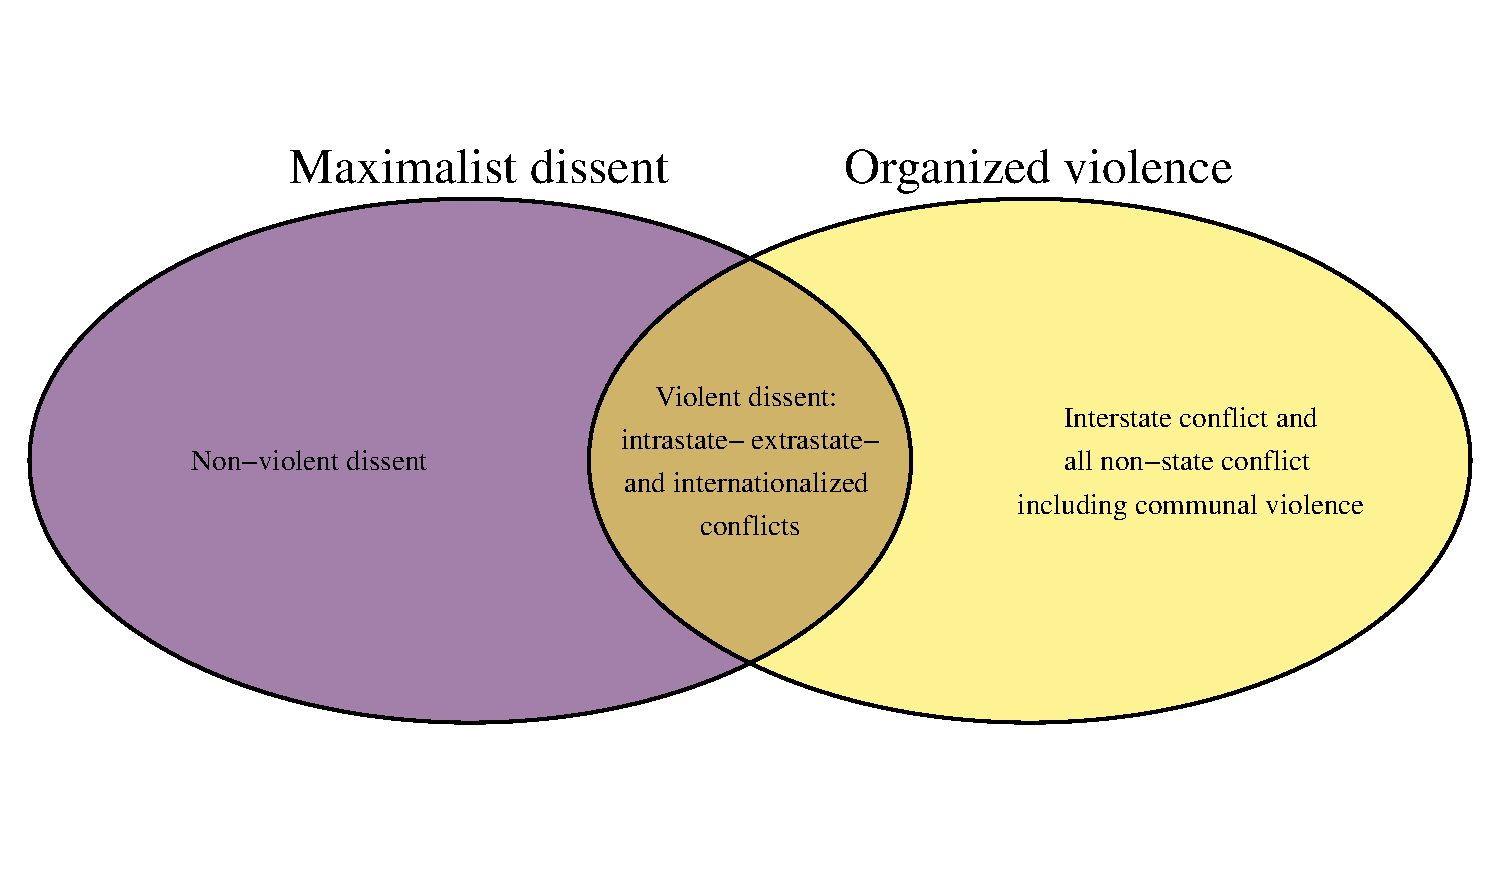
\includegraphics[width=\textwidth]{../R/Output/venn.pdf}
	\caption{Categories of violence and dissent}
	\label{venn}
\end{figure}

\subsubsection{Maximalist dissent} \label{Maximalist dissent}

%Tarrow 1998, `power in movement is cumulative'?

A central concept in the first article of the thesis is maximalist dissent. The
concept builds on \citet{TillyCharles1978Fmtr}'s definition of collective
dissent as observable action involving multiple people, beyond normal
institutional procedures for realizing political goals. This could include
anything from strikes, sit-ins, shirking, large scale demonstrations and other
non-violent tactics, to riots, terrorism or armed rebellion. It does not include
acts of dissent executed in an individual capacity, acts that lack clear
political goals and acts within institutional political bounds (regular
functioning of political parties, lobbying, electoral participation etc.). The
second part of the concept, maximalist, refers to the political goals of the act
(event). The definition builds on the criteria used by the NAVCO 1 data set,
which only includes resistance campaigns where the objective was maximalist
(i.e. regime change, secession, or self-determination) as opposed to limited
(i.e. greater civil liberties or economic rights)
\citep{DVN/0UZOTX/B4RH7S_2019}. The ARC data (presented in Paper I) clarifies
this further as demands that call for changes in the political structure that
would significantly alter the executive’s access to state power, the rules with
which executives are selected, or the policy or geographic areas for which the
executive has the right to make laws \citep{Butcher_2022}.

While the remaining articles of the thesis are concerned with organized
violence, most of which represent the violent part of the spectrum of maximalist
dissent (more on this below), the literature on the non-violent form of dissent
has informed the thesis in a number of ways as well. Understanding how, and
when, nonviolent forms of dissent work and when they do not, can help us
understand when and why people choose to pick up arms and use violence. Several
studies find that nonviolent dissent (or resistance) has a higher success rate
than violent dissent in achieving maximalist political goals
\citep{chenoweth2011civil, Stephan_2008} such as regime change and
democratization \citep{Celestino_2013, Bethke_2019}. Why then do some actors
still chose violence? Part of the answer could be the size of the target
audience \citep{Gleditsch_2021}. Mass mobilization is necessary for nonviolence
to be successful. Goals that benefit a large part of the population, such as
overthrowing an unpopular autocratic regime, facilitate mass mobilization. In
comparison, groups who appeal to more narrow bases such, as self determination
for an ethnic minority, find mass mobilization difficult. For such groups then,
non-violence may not be effective, and so they pursue their goals by violent
means instead \citep{Gleditsch_2021}. Economic structures could matter as well
\citep{Butcher_2014}. A substantial literature is also arguing that repression
of nonviolent campaigns or protests, can cause escalations to violence, although
there is conflicting evidence \citep{Chenoweth_2017, Lichbach_1987}.

Furthermore, a key reason for employing the term maximalist dissent is that
there is no sharp dividing line between violent and nonviolent forms of dissent.
In her study of the civil war in El Salvador \citet{Wood2003} highlights how
rebel groups cooperated and worked closely with civil society, and how
individual rebels shifted between violent and nonviolent forms of dissent. Many
predominantly nonviolent movements have violent wings, who increase the
likelihood of violent escalation -- especially if the nonviolent campaign fails
to make progress \citep{Ryckman_2019}. In Paper I we found that rebel groups
tend to organize in less developed, oil rich countries, while trade unions,
student organizations and other civil society organizations tend to dissent in
more developed countries. This suggest that perhaps some threshold of
development needs to be met in order for countries to have sufficiently well
organized civil society and trade unions to organize for non-violent campaigns.
Perhaps cross national (geographically) and cross societal networks across civil
society must be present similar to what \citet{Wimmer_2018} argues. While rebel
organizations can form relatively locally, especially where opportunity costs of
rebellion are low (low development) and potential gains are considerable (oil
rich country).

\subsubsection{Organized violence}
\label{Organized violence}

\begin{figure}[hbpt]
	\centering
	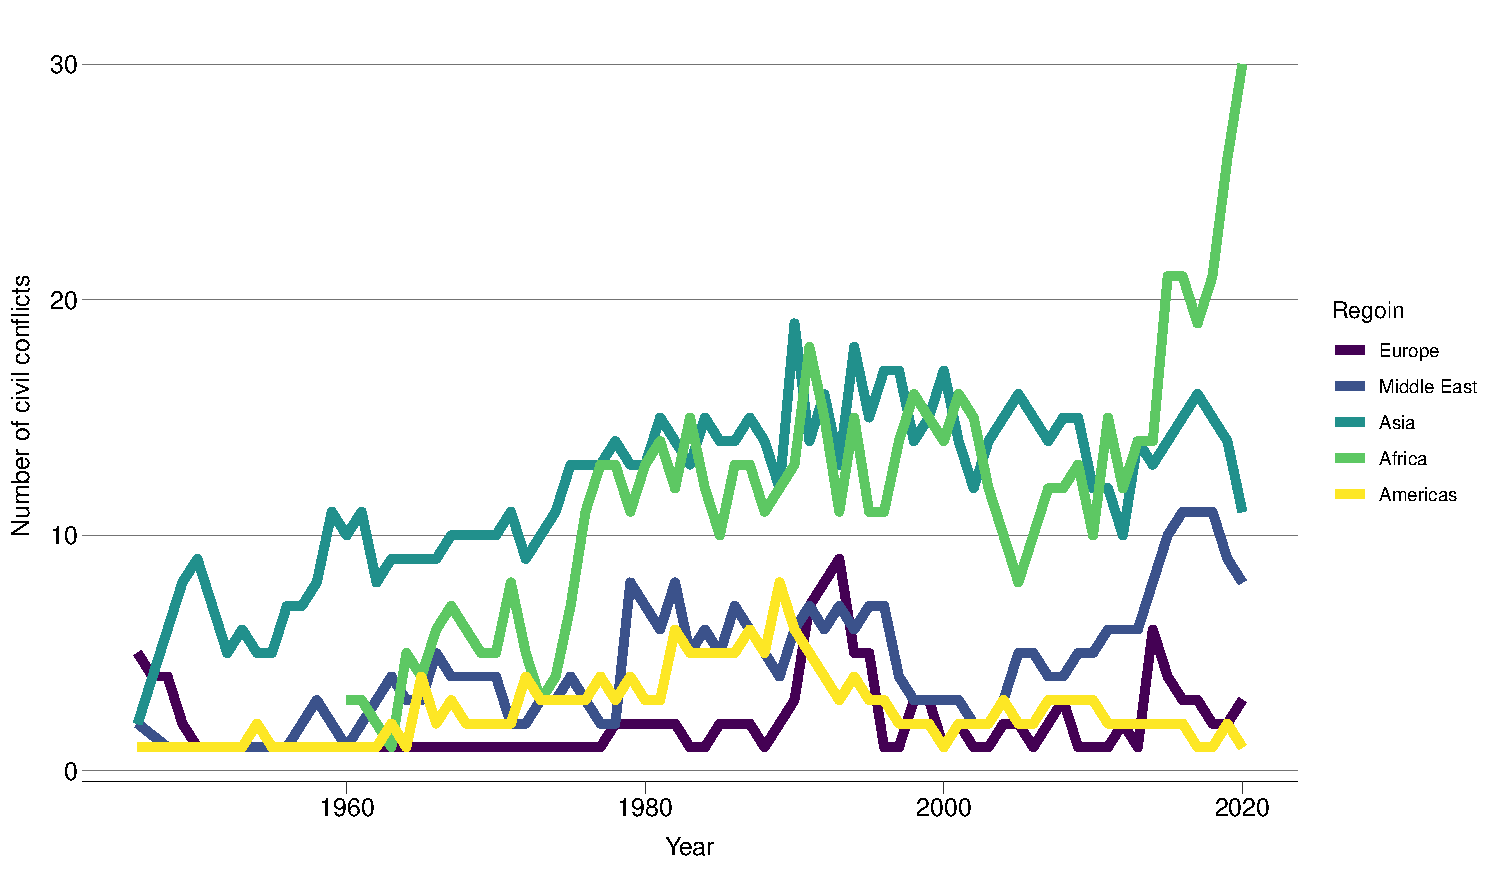
\includegraphics[width=\textwidth]{../R/Output/civilConflictRegion.pdf}
	\caption{Yearly number of civil conflicts per region}
	\label{civilConflictRegion}
\end{figure}

There are many forms of organized violence, most of which are captured by
maximalist dissent. I follow the Uppsala Conflict Data Program (hereafter UCDP)
and \citet{Melander_2016} in treating organized violence as the aggregation of
the mutually exclusive typologies of one-sided, non-state and state-based
violence. One-sided violence is violence committed by formally organised
non-state groups or governments against unarmed civilians. State based violence
is what one usually thinks of as armed conflict, or simply war. More accurately,
it is armed conflict where at least one side is a government (and the other is
not unarmed civilians). This includes inter state conflicts (conflict between
states), extrastate conflict (decolonization-conflicts), intrastate conflicts
(conflicts within states, i.e. civil conflicts) and internationalised internal
conflicts (intrastate conflicts in which at least one party receives troops from
another state). Non-state violence is violence perpetrated by named
organizations (criminal organizations, political parties, rebel groups etc.) or
identity groups (ethnic or religious groups), against one another (without the
involvement of government). Non-state violence therefore is seldom maximalist
dissent, although clashes between political parties or politicised ethnic groups
could be potential borderline cases.

This thesis focuses on two forms of organized violence: civil conflict (which
includes intrastate and internationalised internal conflicts) and communal
violence.\footnote{Historical state entities could matter for interstate
	conflict. For instance in cases where the borders of historical state
	entities cross international boundaries, old borders could form the
	basis of claims making and disputes, such as with the borders of the
	former empire of Bornu \citep{Hariri2012}. However, as in the case of
	Bornu, such disputes can be solved peacefully in international courts.
	Additionally, three of the four papers rely on an African sample and the
	continent have seen only one interstate conflict and no extrastate
conflicts in the time period covered in the papers.} 

\begin{figure}[hbpt]
	\centering
	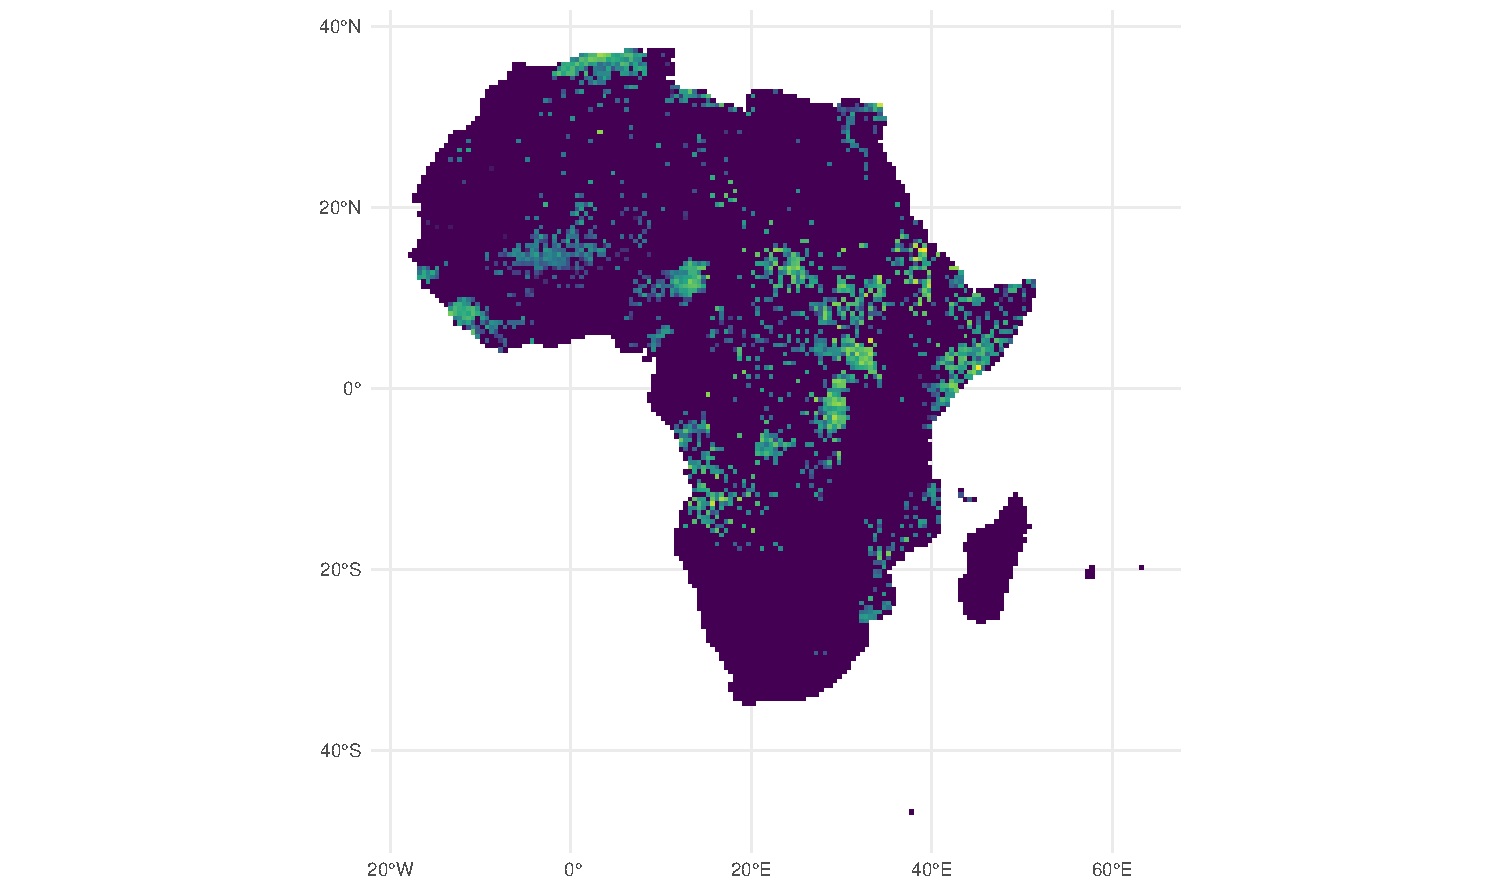
\includegraphics[width=\textwidth]{../R/Output/civilconflictAfrica.pdf}
	\caption{Civil conflict combat related deaths (log-transformed) after 1989.}
	\label{gedAfrica}
\end{figure}

Communal violence is organized lethal violence between identity groups. These
groups can identify along tribal, national, clan, religious, ethnic lines, or
any other source of identity, but are not permanently organized for combat, in
other words not rebel groups, formally organized militias, or state coercive
apparatus. A key difference between communal conflicts and civil conflicts is
that both parties are, at least nominally,\footnote{Gray areas include areas
	outside de facto state control, or cases where one side acts with
government impunity or backing.} subject to the higher authority of the
government in communal conflicts. For further discussion of the concept of
communal conflict see \citet{BroscheJohan2012Cccw}. While events that trigger
such conflicts can be often be relatively minor (theft, trespassing, illegal
grazing etc.) this type of violence tends to quickly spiral through reprisals
and counter reprisals and can generate large death tolls and often far larger
displacement \citep{Horowitz_2001}. 


\section{Theoretical framework}
\label{Theoretical framework}

\subsection{Theoretical traditions} \label{traditions}

There is a substantial body of literature explaining the occurrence (and
re-occurrence) of civil conflict. I broadly divide this literature into three
overarching traditions that continue to inform not only the works presented in
this thesis, but in most of the academic literature on civil conflict. This
literature can be traced back to a handful of classic studies in the 1960s and
1970s. \citet{GurrTedRobert1970Wmr}'s theory of relative deprivation and the
related `revolution of rising expectations' \citep{Davies_1962} focused on how
widespread individual discontent laid the ground for revolution (Section
\ref{Grievance}). This \textit{grievance} tradition of civil conflict was met
with critique from the likes of Charles Tilly and  others, who instead argued
that rebellion happened when there were opportunities for it (Section
\ref{Opportunities}). A more recent branch of the literature builds on models
from microeconomics via international relations theory. Starting from the
assumption that both parties are (usually) best served with a non-violent
bargained solution, this tradition focus on the situations in which bargaining
none the less breaks down, or the exception when conflict becomes a rational
choice (Section \ref{Bargaining}). It should be mentioned that these traditions
are by no means mutually exclusive, and throughout the thesis I draw on each of
them where one might be more illuminating than another. Overall Paper II mostly
draws on opportunity arguments, but also bargaining and grievances (low
development). Paper III  primarily draws on bargaining and opportunity models,
and Paper IV relies partly on grievance models, but also opportunities and
bargaining.

\subsubsection{Grievance} \label{Grievance}

The grievance model of civil conflict originated with
\citet{GurrTedRobert1970Wmr} and \citet{Davies_1962} who emphasized the
discrepancy between expectations of rising living standards and the reality of
stagnation or even worsening conditions. They argued that this \textit{relative
deprivation} among large contingents of society is what drives civil conflict.
This was later expanded on to include structural inequalities as well
\citep{Muller_1985, Muller_1987, ScottJamesC1977TMEo}. For example, the labor
class is experiencing relative deprivation, when they see the wealth they are
generating for the capitalist class, and as a result they are taking up arms.

Responding to the criticism of the opportunities tradition (covered below in Section
\ref{Opportunities}), another branch of the grievance literature shifted the
focus to group level mechanisms, moving away from strict Marxist or materialist
explanations at class or country level. For example, \citet{Hechter_1978} argued
there was a cultural division of labor, and that civil conflict occurred when
cultural and economic groups coincide. Others emphasized competition between
ethnic groups for scarce resources \citep{barth1969}. \citet{Horowitz1985}'s
case studies demonstrated how ethnic groups can garner intense feelings of
belonging, collective self-esteem and group worth, and that ethnic conflict was
not just competition for scares resources, but \textit{also} for political
influence. He anticipated the literature on horizontal inequality by stressing
the role of cognitive comparisons between groups as a mechanism for ethnic
conflict. Despite the scale of Horowitz's study, there was still a lack
systematic empirical support for the idea that grievances (group level or not)
could lead to civil conflict. The drive to address this gap was lead by Gurr and
the minorities at risk (MAR) project \citet{GurrTedRobert1993Mar:}. In response
to Tilly's earlier critique he also added some opportunity to the general
argument of grievance in the resulting work \citep{Gurr_1993}. 

In response to the lack of explanatory power of commonly used measures in the
quantitative literature on ethnicity and civil conflict like ethnic
fractionalization \citep{Alesina2003, Posner2004} and polarisation
\citep{Montalvo2005}, a more recent branch of the grievance literature has
turned to disaggregation in an effort to tighten the logic of causal inference.
This literature has examined  the role of interpersonal grudges and local score
settling in civil violence \citep{Kalyvas2006, Kalyvas_2008}, as well as the
role of moral outrage at government injustice and a sense of doing the right
thing \citep{Wood2003}. Reflecting earlier work by \citet{barth1969}, others who
expressed scepticism of how ethnic identities were used as analytical units in
civil conflict research, they argued that ethnic defection is more common than
previously assumed \citep{Kalyvas_2008, Staniland_2012}, and that ethnic
identities are essentially undetectable or too fluid be of analytical use
\citep{Gilley_2004, Chandra2006}. What is more, the state is not ethnically
neutral \citep{CedermanLars-Erik2013Igac}. Using data from the Ethnic Power
Relations (EPR hereafter) project, \citet{CedermanLars-Erik2013Igac}, building
on previous quantitative efforts \citep{Gurr_1993, Goldstone_2010} were finally
able to put grievances on a solid empirical footing by finding that horizontal
ethnic grievances do increase the likelihood of conflict
\citep{CedermanLars-Erik2013Igac}. 

%[The role of climate and environmental factors \citep{Detges_2017,
%von_Uexkull_2021}] % Grievance or bargaining focused?

\subsubsection{Opportunities} \label{Opportunities}

The main criticism of the grievance literature was the lack for empirical
support for grievance based arguments \citep{Oberschall_1978, Brush_1996}.
Specifically, there seemed to be a discrepancy between the proliferation of
grievances and relatively rare events of civil conflict \citep{Snyder_1972,
TillyCharles1978Fmtr, Skocpol_1979}. Instead, they argue that civil conflict
occurs when groups are able to overcome collective action problems
\citep{Larson_2018}. Thus, research should (according to this branch of the
literature) be focused on finding and examining the contexts in which this
happens.

Seemingly unaware of the critiques that came before them, \citet{Collier2004}
explicitly framed their paper around the `Greed versus grievance' debate and
forcefully reiterated the previous argument that if grievances caused civil war,
then civil conflict would be equally widespread. Instead, they painted a picture
of civil conflict being driven by cynical and greedy conflict entrepreneurs,
arguing that conflict occurs when the potential economic gains from rebelling
outweigh the associated risks. By the time they revisited their
initial article, their framing had become more nuanced, using the term
\textit{opportunities} in the place of greed \citep{Collier2009}. Yet, the
fundamental argument and criticism of the grievance motivated literature
remained largely unchanged. Also writing from the perspective of opportunities,
\citet{Fearon2003} emphasized how fighting in peripheries, rough terrain, state
weakness and corruption due to oil evened the odds in favor of rebel groups,
making them able to challenge the state. Like \citet{Collier2009},
\citet{Fearon_2004} nuanced their initial stance in their follow up work on
civil conflict duration, echoing \citet{WeinerMyron1978SotS}'s `Sons of the soil',
they argued that concentrated peripheral ethnic groups react violently to
perceived incursions. This highlights that these sets of traditions (grievance,
opportunities and bargaining), are not closed categories. Demonstrating a
similar duality, \citet{Weinstein_2005} argued that natural resources provide
opportunities for short term rewards. While in resource poor surroundings, rebel
leaders must make credible promises of future rewards based on political reform,
which is similar arguing that rebel leaders must address economic grievances
(while still employing the theoretical lens and language of opportunities
models).

\subsubsection{Bargaining} \label{Bargaining}

% Relation to opportunities/grievance? Seeking more concrete mechanisms than
% grievance?

\citet{Fearon1995} and \citet{Powell2006} introduced bargaining theory to
international relations. This set of theories starts with the assumption that
war is costly and unpredictable for all parities. Further assuming that actors
are rational, the parties to a disagreement should be able to come to a
bargained solution short of war, to be determined by their relative military
capabilities. \citet{Fearon1995} outlines three basic reasons
conflict might nonetheless occur, aside from breaking or loosening the
rationality assumption. \citet{Pillar_1983} and \citet{WalterBarbaraF2002CtPT,
Walter_1997} and others, introduced bargaining theory to the civil conflict
research,\footnote{See \citet{Walter2009} for a review of bargaining
literature.} and highlighted how characteristics of civil conflict can
exacerbate the three sources of bargaining breakdown.

First, (asymmetric) information problems. Parties have incentives to
misrepresent information about their (military) capabilities, as the outcome of
the bargain depends on the relative capabilities (more relatively capable then
your opponent equals a better deal). The asymmetry between the information about
ones own capabilities and that of the opponent, could lead rational actors to
miscalculate and cause bargaining breakdown by demanding too much or rejecting
offers that would be otherwise acceptable.

Second, commitment problems. In the absence of a third party arbiter and
enforcer, parties have incentives to renege on any bargain that is struck. This
is because if one party demobilizes, and the other does not (reneging on the
deal), the other gains a clear advantage. Thus striking a bargain can be
difficult without mechanisms to ensure that parties make credible commitments
(such as a third party enforcer, or institutional mechanisms). This is (usually)
true both in the anarchy of international relations, but also of civil
conflicts. What makes matters worse in internal conflict is that, unlike
interstate conflicts, only one side usually disarms (rebels) as part of a
negotiated settlement. This makes commitment difficult because once they lay
down their arms, rebels are essentially at the governments' mercy. Additionally,
the government is often fighting multiple rebel groups, which means that
accepting the demands of one group sends a signal of weakness to the others
\citep{Cunningham2006}. This incentives the government to avoid such settlements
and instead push for military victory, and to generally signal willingness to
resort to violence as a means to deter the other actors from making claims
\citep{Walter2006, Walter2009}. Furthermore, rebel groups can easily fracture if
some commanders are not satisfied with the result of the settlement, thus
discrediting the credibility of rebel group commitments \citep{Cunningham2013c}. 
[Anecdote about observing this time and again while coding rebel groups for
ARC?]

Third, issue indivisibility. If the issue of the disagreement does not lend
itself to compromise, for example the issue of slavery in the American civil war
(you cannot have just a little slavery), finding a bargain that reflects the
relative capabilities is difficult. Interstate conflicts over territory can (at
least in theory) be resolved by territorial concession matching the relative
capabilities of two warring states. On the other hand when rebel groups fight
for secession or regime change, finding some level of concessions that match the
relative capabilities becomes much more difficult because of the
winner-takes-all nature of the issues common to civil conflicts \citep{Toft2005,
Duffy_Toft_2002}. 

%\citet{Denny2014} Unifies all! Ethnic groups are likely to have grievances, are
%better able to organize (opportunity) and are more likely to face bargaining
%issues.

\subsection{The Janus face}
\label{Janus}

%Some more prior literature: \citet{Griffiths2016} \citet{Ahram2019}

Drawing from these theoretical traditions, I build a new theory of how
historical states shape conflict and peace in the modern world. The main
argument of the thesis, and its main theoretical contribution, is that the
relationship between historical statehood and organized violence is conditional.
On the one hand, it can be a force for peace, but on the other it can be a
source of conflict. This conditionality helps make sense of the seemingly
contradictory findings in the existing literature. The conditions determine
which of mechanism become relevant, as outlined in Figure \ref{Mechanisms and
modifiers}.

\begin{table}[hpbt]
	\begin{tabularx}{\textwidth}{>{\centering\arraybackslash}X>{\centering\arraybackslash}X>{\centering\arraybackslash}X}
	\textbf{Condition} & \textbf{Mechanism} & \textbf{Outcome} \\
\toprule
	\multirow{4}{=}{\centering{Number and far from capital}} & Symbols & \multirow{4}{=}{\centering{Conflict}} \\
    	\cmidrule{2-2}
	& Claims making groups & \\
    	\cmidrule{2-2}
	& Colonialism, democracy and weak statehood & \\
	\cmidrule{2-2}
	& Elite networks & \\
	\midrule
	Near to capital & Security apparatus & \multirow{5}{=}{\centering{Peace}} \\
		\cmidrule{1-2}
	\multirow{3}{=}{\centering{Type of violence}} & Enforcement of contracts
						      (in the past) & \\
		\cmidrule{2-2}
	& Resolution of disputes (in the past) & \\
		\cmidrule{2-2}
	& Forceful reduction of internal conflict (in the past) & \\
	\bottomrule
\end{tabularx}
\caption{Mechanisms and modifiers}
\label{Mechanisms and modifiers}
\end{table}

Despite having lost their sovereignty, old states do not disappear without a
trace. This thesis rests on the argument that historical states can leave behind
symbols, elite networks, institutions and a legacy of reduced intercommunal
violence. 

I use the term `symbols' as a deliberately vague term to describe the practical
application of the collective memory of historical states. In other words, when
the collective memory of some past state is invoked by someone to serve some
purpose, it is used as a symbol. The purpose of using such a vague term is that
different states can produce different collective memories, which can be used by
different actors in different ways. `Symbols' is thus meant as a catch all term
for something that is too complex to disaggregate (at least in the context of
this thesis). Primarily such symbols are useful for generating group cohesion
(potentially by delineating a clear in group as opposed to the out group), and
for conferring legitimacy.

The elites, that states produce, cultural, economic, political or religious,
rarely disappear along with the sovereignty of the state. Instead, they are
either incorporated into the new state, or are transformed to regional or
local elites. As evidenced by a number of case examples throughout the thesis,
the social networks of these elites can be remarkable stable over time, and can
span multiple generations.

Institutions often survive into new states as well, either as formal or informal
institutions. `Institutions' is once more a purposefully vague term which can
describe leaders, courts, councils, laws et cetera. The reason for using such a
vague term is, as with symbols, to capture a general, yet distinct, phenomenon
that is too complex to disaggregate.

None of these legacies are inherently conflict inducing. While symbols can be
used for mobilization, they can just as well lend legitimacy to the central
state, or facilitate public goods provision through shared identities. The
organizational capacity of elite networks and institutions can be used for both
violent mobilization or better governance. However the effect of historical
state legacies are conditional, and these legacies only become conflict
inducing, or peace promoting in combination with other factors.

\subsubsection{Distance to capital} \label{dtc}

The distance between the capital and a pre-colonial state matters because it
proxies the relationship between the pre-colonial state and the central, or
post-independence state, and the relative military capabilities between them. If
a pre-colonial state is close to the capital there is a good chance that its
institutions, elites and main ethnic group are well represented in government,
if not its main component.\footnote{For example most of the North African states
Merina in Madagascar or Ouagadougou in Burkina Faso.} In other words it is
unlikely that the potential conflict inducing capabilities of the pre-colonial
state will be used against the central government. Instead it is a potential
source of peace promoting mechanisms such as legitimacy, institutions such as an
experienced security apparatus and institutions useful for bargaining.

On the other hand, far from the capital the relationship between pre-colonial
state elites, institutions and ethnic groups are more likely to take the form of
a center-periphery cleavage \citep{1967Psav}. In this scenario, institutions,
elite networks and unifying symbols of a past statehood can translate into
potential to mobilize against a central government. For example, rebel groups
use the symbolic effect and collective memory of past states as focal points for
mobilization. This is often displayed prominently in the names of various rebel
organizations,\footnote{Examples include The Macina Liberation Front, Al
Mourabitoun, Cyranecia Liberation Army and the Free Ache Movement.} or is a
common feature of their manifestos or ideological writings. What is more, states
create hierarchical, or vertical, social networks that often persist for
generations, long past the death of the state. In a new state, former national
elites become new regional elites. Given the increased likelihood of indirect
rule, regional elites created by past states are often more autonomous. Recent
work by \citet{Ying_2020} suggest that one source of conflict outbreak is when
the state expands its influence into areas which previously enjoyed regional
autonomy. The vertical nature of these social networks also makes them better
able to mobilize. 

Crucially, being far away from the capital evens the relative capabilities
between prospective challengers and the state, which increases the danger of
miscalculation. This danger is exacerbated by the fact that information
deteriorates over distance as well, further increasing information asymmetries.

Past statehood gives peripheral groups opposing the central government another
key advantage over other groups. Given the importance of the sovereignty
principle in the international system,\footnote{Article 2.1 of the United
	Nations Charter reads: `The Organization is based on the principle of
the sovereign equality of all its Members.'} wherever there are historical
states, their past sovereignty can form the basis of claims making for ethnic
groups tied to past states. What is more, states can both create and spread
ethnic groups over large geographical ares, and thus potentially be the source
of politically relevant ethnic groups in multiple countries. 

\subsubsection{Number of HSEs} \label{Number of HSEs}

The number of historical state entities matters for two reasons. First, more
historical state entities increases the likelihood that one or more of them are
far from the capital and thus might trigger the above mentioned mechanisms.
Second, it adds two conflict inducing mechanisms of its own. Having more of
areas with such qualities within the boundaries of a country, in and of itself
raises the likelihood that one or more of them will eventually challenge the
state. However, in addition it creates an incentive for the government to signal
toughness and resolve (as explained in Section \ref{Bargaining}). The other
mechanism is that, where strong states existed they more often resisted
colonization, and when they were colonized were more likely to be ruled
indirectly \citep{Englebert2000, Gerring2011, Hariri2012}. This meant that such
ares were more likely to preserve existing autocratic ways of rule, and to a
greater extent resisted the influence of western ideas of democracy and modern
bureaucracy. Thus they circumvented the peace inducing effect of democracy, and
were left with less effective institutions.

\subsubsection{Conflict type} \label{Conflict type}

Finally, the effect of pre-colonial statehood does not have the same effect
across categories of organised violence. As elaborated in Section \ref{Communal
violence}, communal conflicts are distinctly different from civil conflicts. For
one they are horizontal rather than vertical in nature. So while pre-colonial
states affects the relationship between groups with ties to that state and their
central government in one way, it might change the ways those people interact
with other groups in quite different ways. Specifically, in Paper III, we argue
that in their domain, states leave a legacy of reduced intergroup violence,
through enforcing contracts, resolving disputes and forcefully reducing internal
conflict when necessary. In other words, the pre-colonial state facilitated
bargaining between groups by acting as an arbiter. The initial reduction sets in
motion a positive feedback loop of increased interaction and trade between
groups, which makes punishing spoilers\footnote{Someone whose individual gains
	of spoiling the bargain (peace) exceeds that of continued cooperation.
	In the absence of intergroup interaction, a member of one group can
	commit crimes, such as a cattle raid, against the other group, and hide
in anonymity amongst his own group. Any punishment by the aggrieved party will,
in the lack of means to identify the thief, be carried out collectively against
his group, and so communal conflicts ensue.} individually, rather than
collectively, possible. The stronger the presence of the pre-colonial state, the
more effective the initial reduction of the security dilemma and commitment
problem between groups, and thus the larger the degree of intergroup interaction
and trade, further reducing the information problem. In the paper we even show
that pre-colonial state presence positively correlates with ethnic
fractionalization. This is consistent with our hypothesis that pre-colonial
states have reduced communal violence in the past, and that this has indeed
facilitated increased intergroup interaction to the point that groups feel safe
enough to settle amongst each other.

%[Where to put this table \ref{Conditional effects}? Remove it?]
%
%\begin{table}[hpbt]
%\begin{tabularx}{\textwidth}{>{\centering\arraybackslash}X>{\centering\arraybackslash}X|>{\centering\arraybackslash}X|>{\centering\arraybackslash}X}
%    & & {Low levels of state presence} & {High levels of state presence} \\
%\midrule
%     \multirow{2}{=}{\centering State based violence} & Near capital & Conflict &  Peace \\
%     \cmidrule{2-4}
%					   & \makecell{Far from \\ capital} & Peace & Conflict \\
%\midrule
%     \makecell{Communal\\ violence} & & Conflict & Peace \\
%\end{tabularx}
%\caption{The conditional effects of historical statehood}
%\label{Conditional effects}
%\end{table}
% }}}

\section{Analytical approach} \label{Analytical approach}

% Data narrative (inductive/deductive). Empirical tradition.

The analytical approach of this thesis is quantitative in nature, and seeks to
uncover generalizable (across the relevant sample), probabilistic relationships.
Doing so requires statistical data, and much of the novelty of this work lies
the data assembly that was done as part of this thesis. Both as part of the ARC
project, released as Paper I of this thesis, but primarily the Geo-ISD which
forms the basis of papers III and IV. The following sections will focus on the
latter.

\subsection{Data on historical statehood} \label{Data on historical statehood}

% Wig only dyadic and only ethnic conflict.
% Both rely on the Murdock map and EPR

% DP LARGE grid cells, limited sample of states and state borders, strange
% measure of conflict (proportions of years with ANY type conflict).

% Paine Limited sample of states leads to no country has multiple state groups

%Going from the ISD to EJIR article. Using existing data in new ways/staring from
%a different (non-ethnic) point of view.

%%%%%%%%%%%%%%%%%%%%%%%%%%%%%%%%%%%%%%%%%%%%%%%%%%%%%%%%%%%%%%%%%%%%%%%%%%%%%%%%

As mentioned previously, the literature on the legacies of historical statehood
has been somewhat limited by the availability of data on historical statehood.
Most previous studies use a combination of two sources (with some efforts to
build on these). Namely, the Murdock map \citep{Murdock1967} and the State
Antiquity Index \citep{Bockstette2012}. While both have unique shortcomings, a
common weakness is that they miss a substantial number of historical state
entities, particularly in Africa. Second, neither contain accurate data on where
the included stats were present. The Murdock map \citep{Murdock1967} only
provides a measure of the `stateness' of ethnic groups.\footnote{Measured as
jurisdictional hierarchy ranging from none to kingdom and Empire.} Tying this
measure to the geographical settlement of ethnic groups (past or present) builds
on some questionable assumptions. The State Antiquity Index for its part
aggregates state histories to current country level. The differences between
native and colonial state experience, and variations across time (duration of
the state) and space are addressed using a weighting scheme.

In Paper II using the ISD (version 2) rectifies three of the common shortcoming
in the literature on historical statehood and civil conflict
\citep{Griffiths2013}. First, the ISD is a global sample, and thus avoids the
African bias in this literature. Second, and partially related, we move beyond
ethnic groups as the unit of analysis. Third, the ISD identifies far more states
than comparable data efforts,\footnote{439 unique states.} and does so starting
from a definition of state that does not require [arbitrary][too strong, what's
a better word?] conditions such as recognition by one or more European power
\citep{Griffiths2013}. [More detail on the ISD? Feel like I do that elsewhere]

\begin{figure}[hpbt]
	\centering
	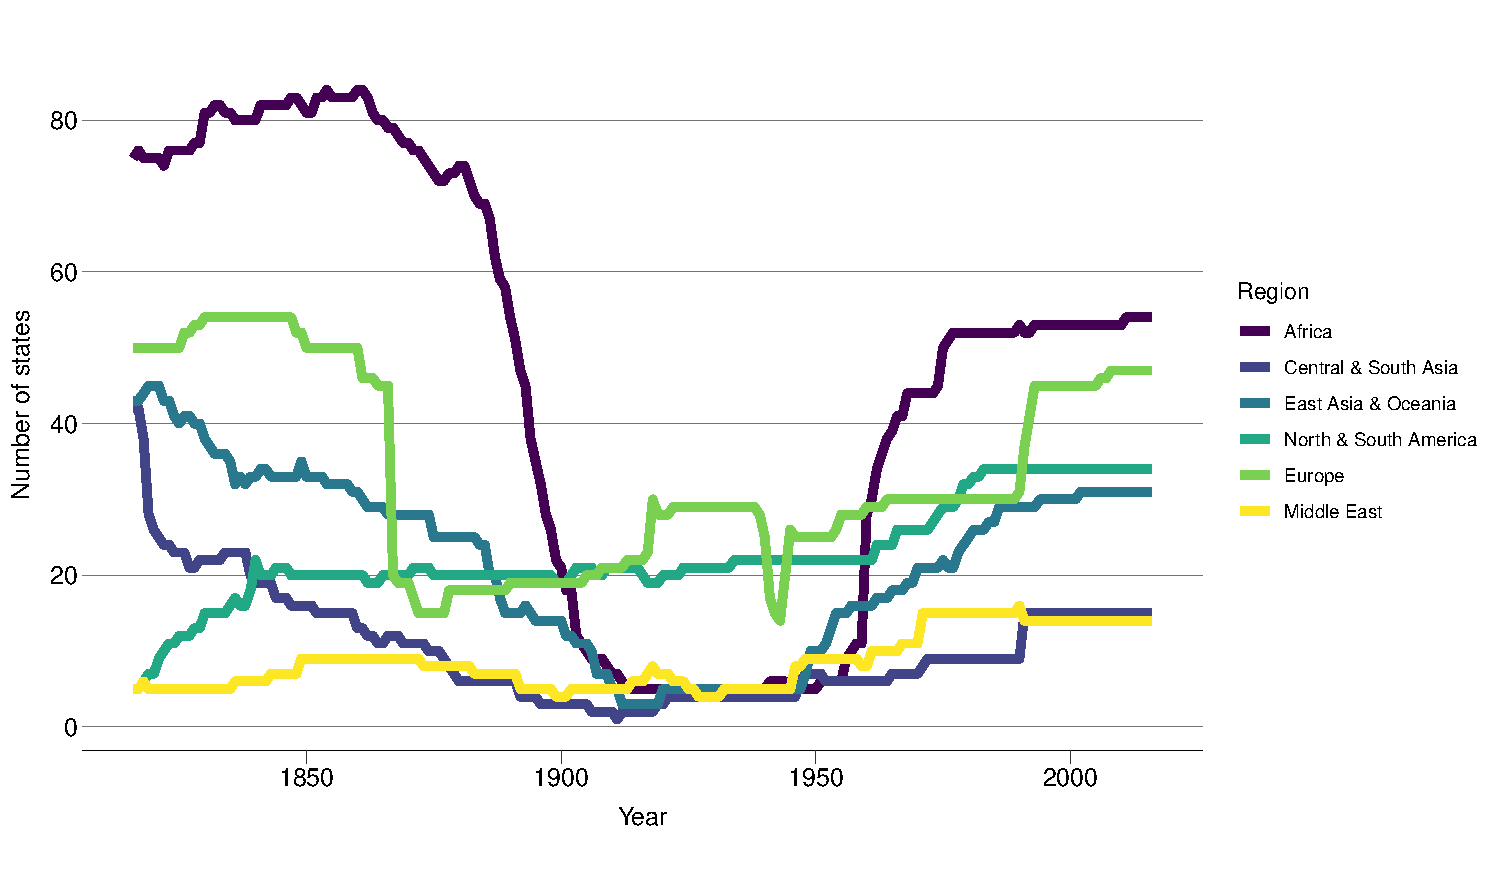
\includegraphics[width=\textwidth]{../R/Output/statesPerYear.pdf}
	\caption{The number of independent states per year.}
	\label{statesperyear}
\end{figure}

Building on the State Antiquity Index, \citet{Depetris-Chauvin2016} (to my
knowledge) represents the only previous attempt to create a measure of
historical state presence disentangled from ethnic groups and current countries.
However, as with the State Antiquity Index and Murdock map, his data only
contains the most well known African states. While avoiding aggregating to
current country boundaries, the data is nevertheless highly aggregated at a
2\degree  by 2\degree  grid cell level.\footnote{Approximately 222 by 222
kilometers at the equator.} Finally, the data do assume that states have uniform
control, or degree of presence, across a constant set of `hard' boundaries for
half century periods \citep{Depetris-Chauvin2016}. 

The Geo-ISD seeks to build on the advance made by  \citet{Depetris-Chauvin2016}
in creating a measure of historical statehood that is untangled from ethnic
group and modern boundaries, by making use of a grid cell representation of
state presence. In addition, the Geo-ISD seeks to address the three shortcomings
of the data, namely: number of included African states, high level of
aggregation, and assumption of uniform state presence across territory.

\subsection{Geo-ISD: moving beyond two dimensions} 
\label{Geo-ISD}

Prior to the globalisation of the Wesphalian model, drawing a discrete line on a
map is not an accurate way to depict what is, and is not part of a state. The
extent of states, would vary according to their ability to project military
power outside an alluvial core, surrounded by a large, permeable frontier. State
penetration into the frontier was in the form of relations with groups, ranging
from tributary, through allied or hostile to extracting `protection' payments
from the state \citep{Scott2009}. In fact, by some accounts the vast majority of
people lived outside states until at least 1600 \citep{scott2017against,
Scott2009}. In many parts of the world, this was still the reality in the
nineteenth century \citep{Scott2009}. Boundaries between states, where they
occurred, were usually in the frontiers of each state, where neither would have
full control. Any attempt to depict the geographic extent of states in such a
pre-Westphalian state system, should take this gray-area of the frontier into
account. A more accurate representation would be a gradient of statehood that
fades into the frontier, for most of Africa and Asia in the nineteenth century.
Roughly conforming to concentric circles extending from a core area. The Geo-ISD
to create such a measure of statehood, which captures geographic extent in
addition to depth, termed `state presence'.

[Struggling with balancing this vis-a-vis Paper IV which has a lot on the
Geo-ISD. Will try to be brief on the parts covered in the paper and expand on
stuff that was not included there. What is missing from the paper? I feel like I
got most of it in there now that we decided on `big impact' paper]

[What NEW visualizations of the Geo-ISD could I do?]

%TODO: redo this with viridis and better resolution pdf
\begin{figure}[hbpt]
	\centering
	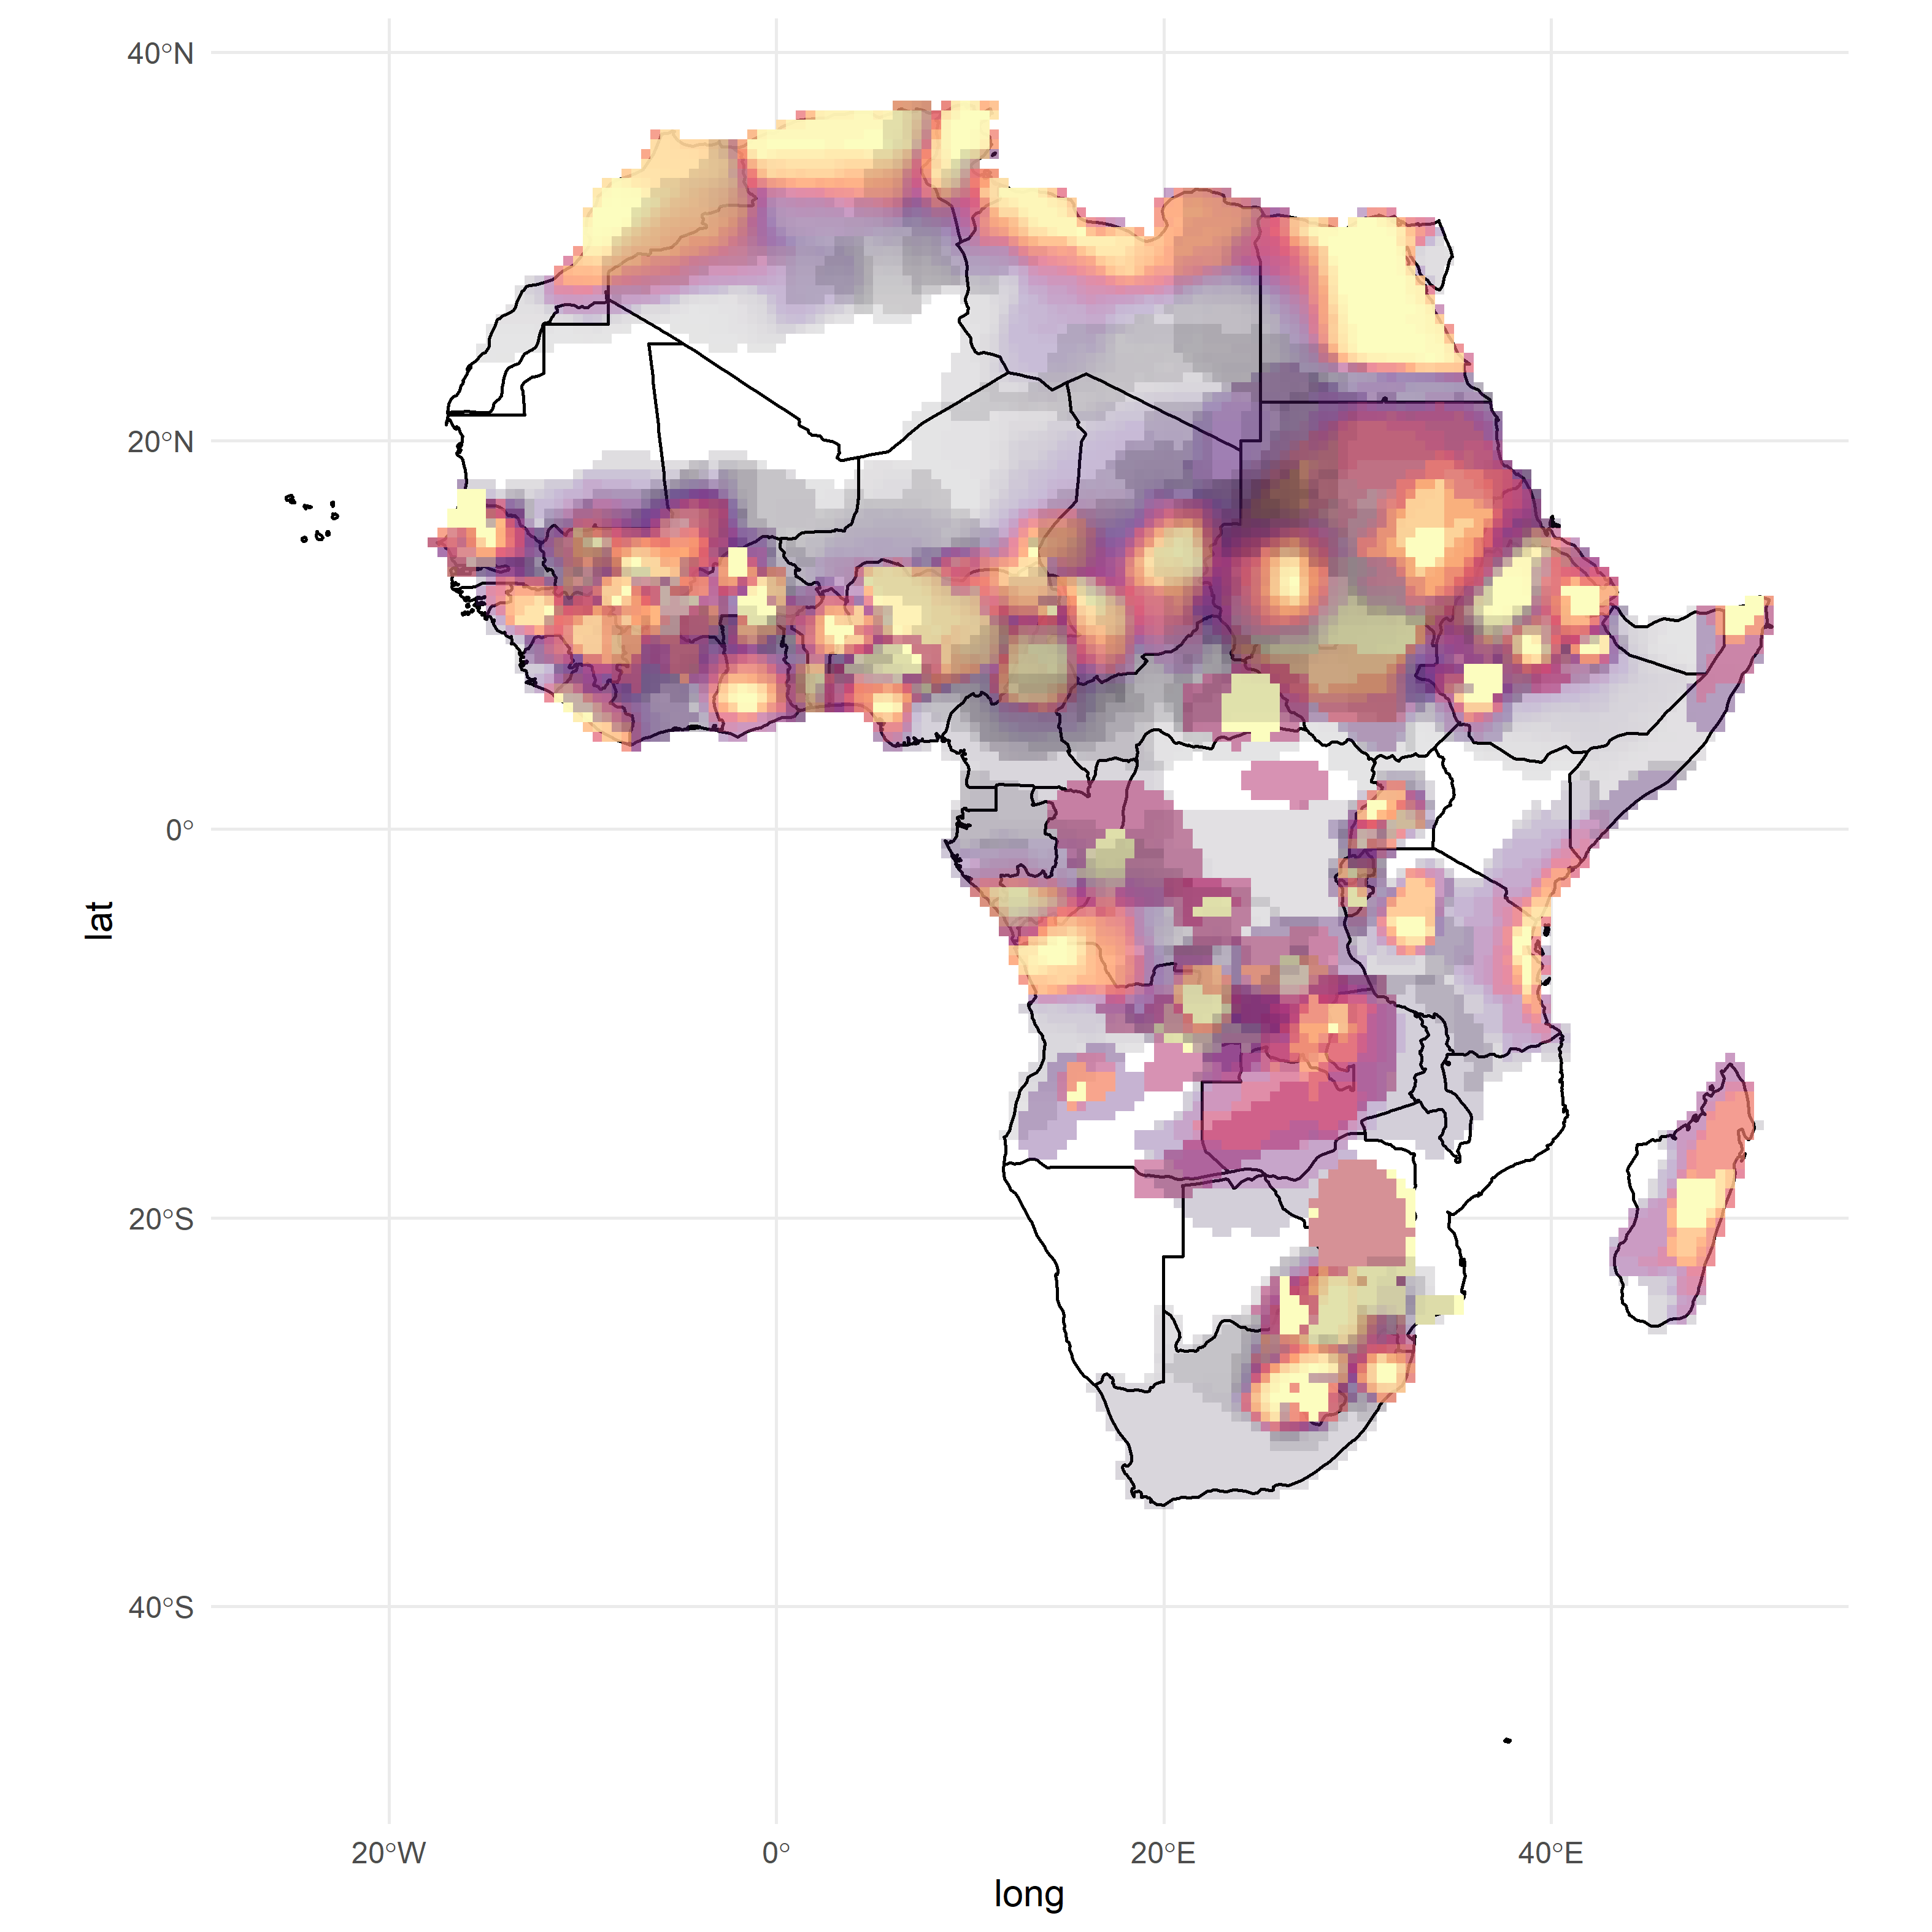
\includegraphics[width=\textwidth]{img/geo_isd_all.png}
	\caption{Pre-colonial state presence (normalized per state)}
	\label{spnorm}
\end{figure}

As the name implies the Geo-ISD builds on the identification work of the ISD,
and follows its definition of state. To this, the Geo-ISD adds geocoding of
state presence for Africa. To construct this measure the Geo-ISD primarily
relies on historical maps from the David Rumsey project, covering the 1800-1914
period, complimented by historical atlases compiled by later historians. The
maps from the David Rumsey project typically depict the `current' political
[situation] to the best of European map makers knowledge. The Geo-ISD leverages
the variations in this knowledge and the differences in the conceptualisations
of statehood that led the map makers to draw the political lines on the map
exactly where they did. For example, one might include vassal states as part of
a kingdom, while other would not, and yet others would include some vassals, but
not others. The pre Westphalian international system had ample grey areas for
such variation to manifest. Indeed there is an almost continuous range of
possible degrees of sub state sovereignty/independence, from fully subordinated,
core areas of states to being subjugated only in name while receiving tribute
from the nominal overlord. Nevertheless, all maps should agree on where the core
areas of states were, and moving away from the core, gradually fewer maps would
consider these peripheries as part of the state. Similarly, the cases where
mapmakers disagree on whether or not some realm qualified as a state, it
reflects that it lacked the institutions or political centralization to have
much presence as a state. By aggregating we leverage both these variations in
conceptualizations of statehood as well as variations in \textit{actual state
presence} over time, as kingdoms and empires influence [ebbed and flowed].

The end result is a three dimensional,\footnote{Latitude, longitude and `depth'}
continual measure that I argue more accurately [tracks/depicts] the
pre-Westphalian international system in Africa from 1800 to 1914. Figure 5.3 in
Paper IV displays the resulting data. 

However, the Geo-ISD also provides information on borders that I do not analyze
further in this thesis. For example, a measure of `frontierness', the degree to
which an area has had one or more border crossing it (Figure \ref{fig:borders}),
or a measure of `borderlandness', the degree of overlapping sovereignty (how
often \textit{more than one} state's borders cross an area)(Figure
\ref{fig:overlaps}). 

\begin{figure}[hpbt]
	\centering
	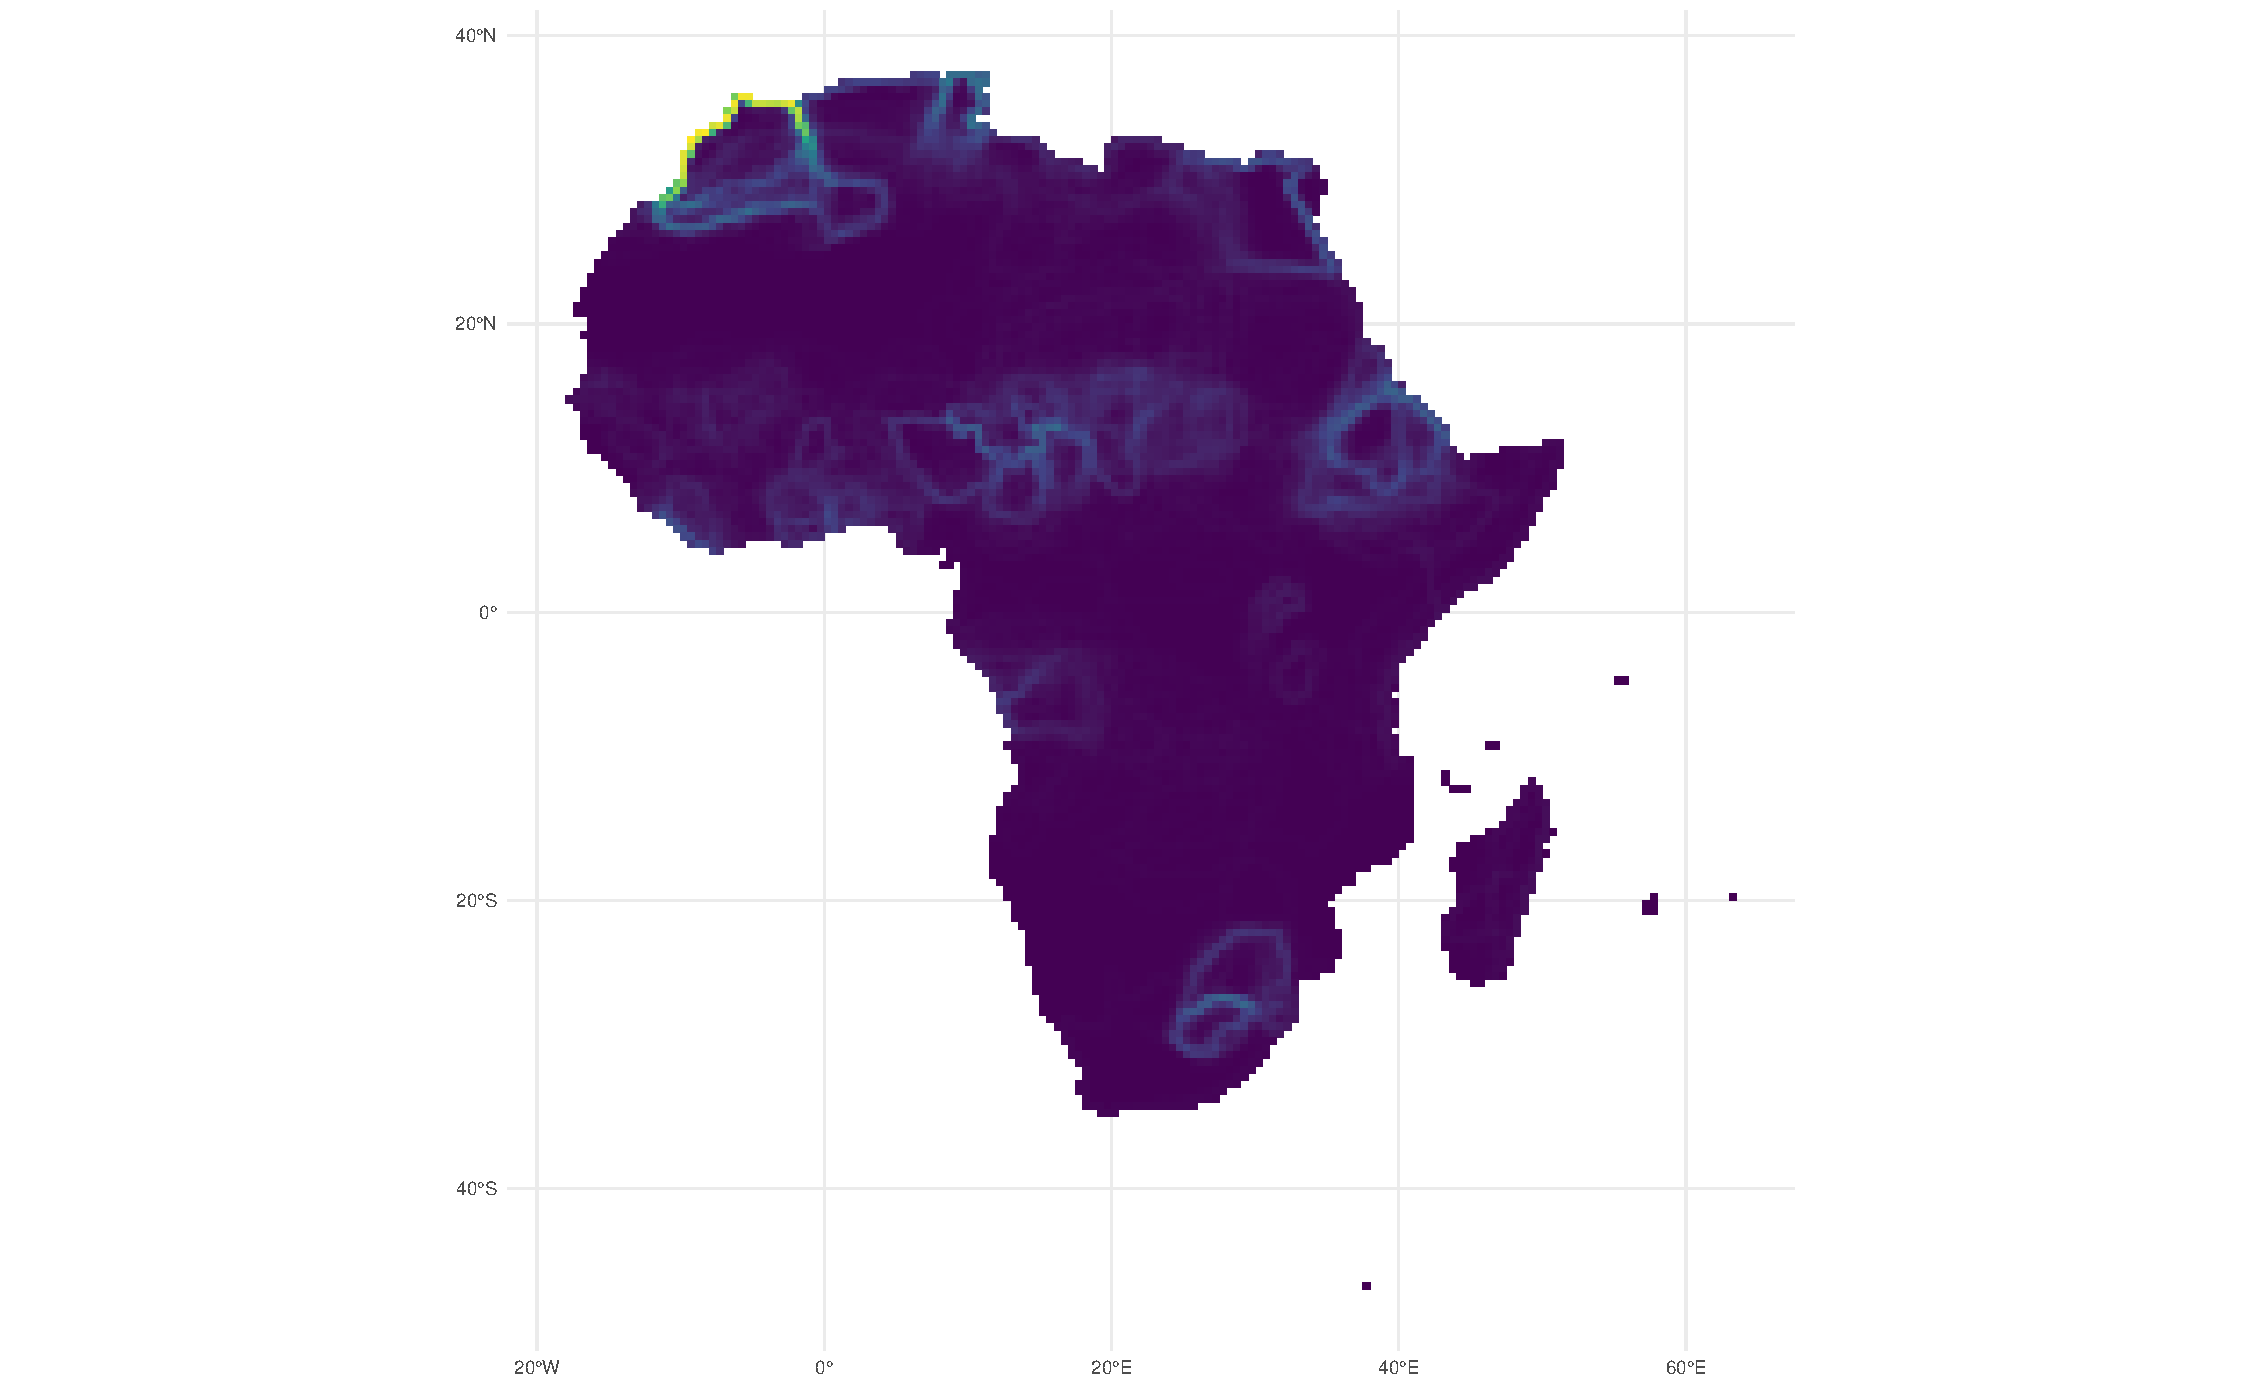
\includegraphics[width=\linewidth]{img/sp_b_sum.pdf}
	\caption{`Frontierness', the number of borders (log).}%
	\label{fig:borders}
\end{figure}

\begin{figure}[hpbt]
	\centering
	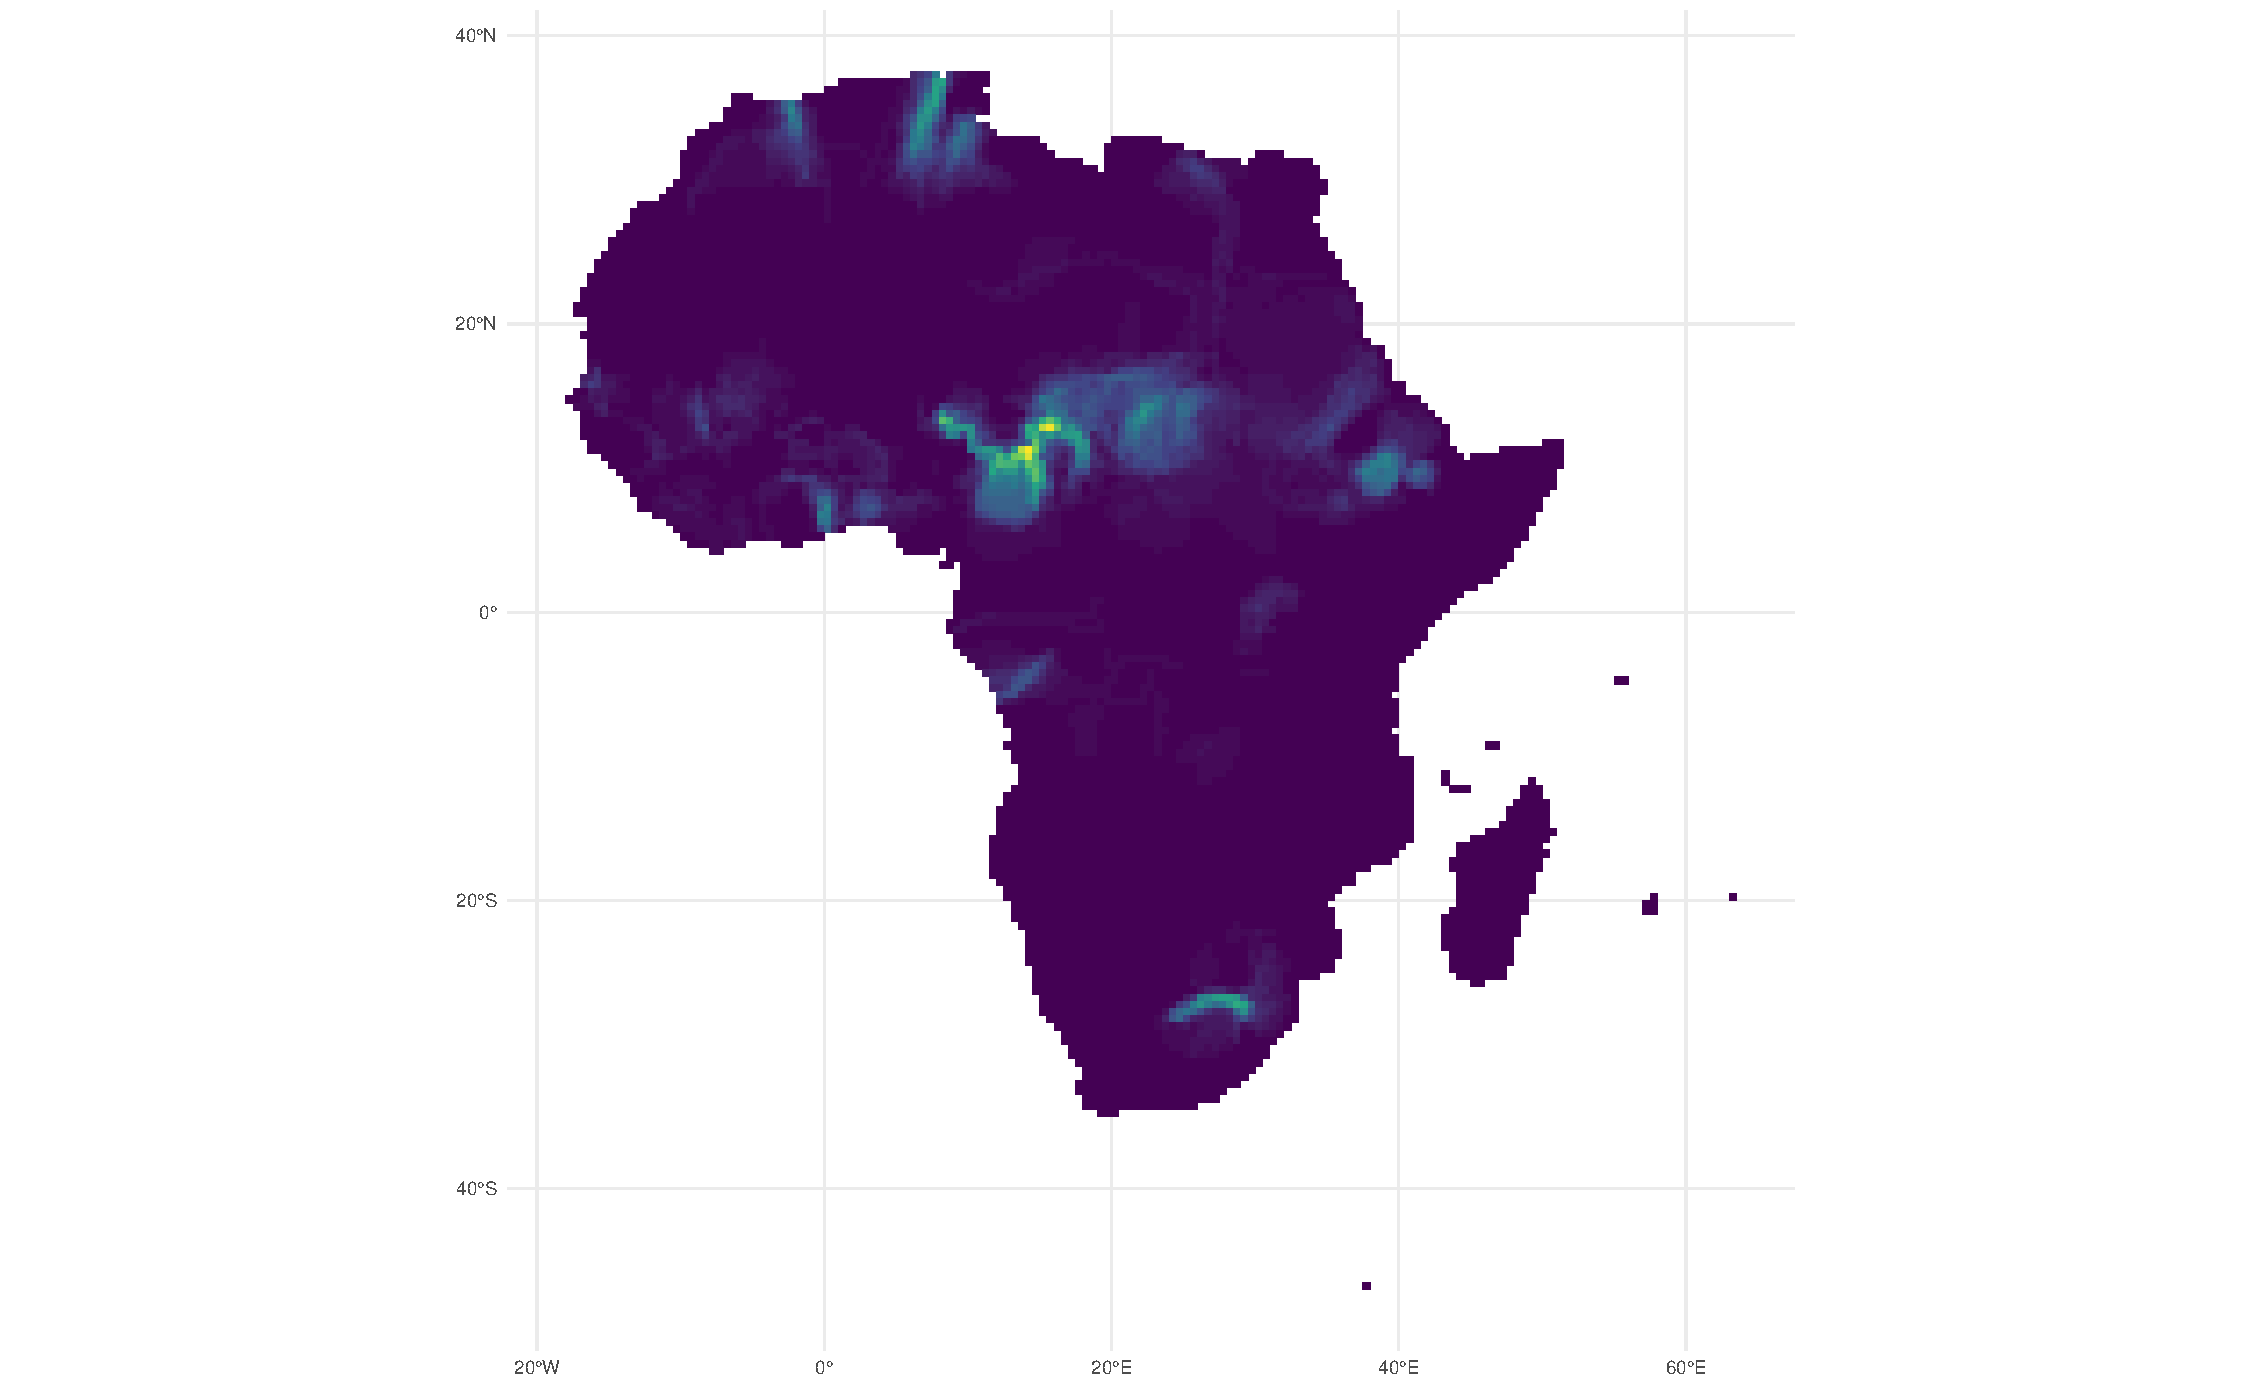
\includegraphics[width=\linewidth]{img/sp_o.pdf}
	\caption{`Borderlandness', the number of border overlaps (log).}%
	\label{fig:overlaps}
\end{figure}

\section{Article summaries} \label{Article summaries}

\subsection{Paper I: Introducing the Anatomy of Resistance Campaigns (ARC) Dataset}
\label{Paper 1}

Published in: \textbf{Journal of Peace Research}\\
Co-authored with: \textbf{Charles Butcher, Jessica Maves Braithwaite,\\
	Johnathan Pinckney, Eirin Hauseth and Ingrid Vik Bakken.}\\

While the literature on resistance campaigns has long emphasized the role of
organizations in overcoming collective action problems, mobilizing for
campaigns, and effecting the outcome of campaigns \citep{Braithwaite2020,
	Brancati2016, Butcher_2014, Celestino_2013, chenoweth2011civil,
HaggardStephan2016DaD:, TarrowSidneyG.2011Pim:}, until recently there has been
little data on organization types, goals and the connections between them. Paper
I is a data release paper for the Anatomy of Resistance Campaigns project
(ARC-project), which seeks to address this lack of organization level data. In
it we present detailed data on 1,426 organizations that engaged in maximalist
dissent in Africa during the 1990-2015 period. The data covers 17 organization
features including type, goals, leadership, origin and social base, in addition
to ties to other groups (see \ref{Tab: Table 1} for full list of features). This
allows the mapping of inter organizational networks of alliances (horizontal) and
fronts (vertical).

The paper also tests correlates of organizational participation, and finds that
rebel groups tend to mobilize in poor countries while trade unions, student
organizations and other civil society groups are more common in developed
countries. These results are in line with both opportunity costs and poverty as
grievance explanations of civil conflict \citep{Collier2009, Davies_1962,
GurrTedRobert1970Wmr}. They also support modernization theories of
democratization \citep{Butcher_2014, Dahlum2019}. In terms of interconnectedness
the article finds that rebel groups (perhaps unsurprisingly) tend to cooperate
amongst each other, rather than with other type of groups.\footnote{To the
degree that other groups cooperate with rebel groups they tend to do so
clandestinely rather than overtly. Thus, it is difficult to capture and perhaps
underrepresented in the data.} Political parties, trade unions, and civil
society organizations tend to form fronts and cooperate with one another, while
religious organization cooperate more narrowly with other civil society
organisations.

\subsection{Paper II: Beyond Ethnicity: Historical States and Modern Conflict}
\label{Paper 2}

Published in: \textbf{European Journal of International Relations}\\
Co-authored with: \textbf{Charles Butcher}

In Paper II we argue that the more historical states are confined within the
boundaries of a country the more likely civil conflict onsets become. This is
because each historical state entity has four potential mechanisms leading to
civil conflict, and the more there are, the more likely it is that one or more
mechanism triggers. First, historical states created elite networks useful for
insurrection. Second, they provide likewise useful symbols of past sovereignty.
Third, states generated and spread modern ethnic groups that, once part of a
larger state, activated dynamics of ethnic inclusion and exclusion. Fourth,
states were typically more able to resist colonization than non-state areas.
While most of the was colonized, states were more likely to be so indirectly.
The stronger the state the more autonomy they were able to hold on to. However,
resisting colonization also meant resisting western ideas of government,
enlightenment and democracy, which in the long run have had peace inducing
effects. We also find that conflict onsets are more likely when historical state
capitals are located far from the current capital, and the effects are stronger
in less developed countries. We argue that the latter is due to more developed
state being better able to incorporate other states.

For the analysis we used the ISD version 2 which records independent states
between 1816 and 1939, where `independent state' is defined as polities that
have more than 10,000 people, autonomy over a specific territory and uncontested
or recognized external sovereignty \citep{Butcher2020}. For determining which
current country historical states are in, we use the approximate location of the
historical state capital, also included in the ISD. To capture the missingness
that this creates when historical states overlapped current boundaries, we
supplemented the initial count with data from the World Statesmen database of
traditional states. A key benefits of using the ISD is its global coverage and
that it does not select on ethnicity, both of which are features that several
studies in the field do not have. 

\subsection{Paper III: Communal Violence and the Legacy of Pre-colonial States}
\label{Paper 3}

Co-authored with: \textbf{Ole Magnus Theisen}

Paper III addresses how pre-colonial state presence affects communal conflicts.
Unlike for civil conflict, we find that state legacies have a conflict reducing
on communal violence. We argue that pre-colonial states initially reduced the
security dilemma and commitment problems between groups, by forcefully reducing
intergroup violence and acting as a third party enforcer of contracts. This
initial reduction of violence allowed for virtuous cycles of increased
interaction and trade between groups, which reduced information problems and
increased the long term pay off of cooperation relative to the short term pay
off of defection. We find empirical evidence of this mechanism in increased
ethnic fractionalization in areas with more pre-colonial state presence.
Indicating that pre-colonial states, despite their shallow presence relative to
modern states, did allow for a greater degree if interaction between groups. The
finding that pre-colonial states reduce communal violence is also consistent
with the argument in the literature that conflict reducing institutions have
been persistent in many cases \citep{Wig2018}. This is the first paper to use
the Geo-ISD data on pre-colonial state presence.

\subsection{Paper IV: After Forever: Pre-colonial States and Civil Conflict}
\label{Paper 4}

The last paper of the thesis is the one that most directly addresses the
overarching research question of the thesis of how historical state legacies
affect long term levels of organised violence. By using the pre-colonial state
presence measure from the Geo-ISD, this paper compliments Paper II of the thesis
in two ways. First, it re-examines the relation between pre-colonial/historical
states and civil conflict, but at a grid cell level, as opposed to country
level, and by using a continuous measure of state presence, rather than a count.
Second, like in Paper II I emphasize the distance to the current state capital.
However, Paper IV goes beyond that by examining how distance to the capital and
pre-colonial state presence \textit{interact} to affect civil conflict both to
reduce and induce violence. I argue that pre-colonial state presence has a
conflict reducing effect when close to the post-independence capital because the
short distance means that traditions, elite networks/elite cohesion and
institutions are at the disposal of the central state. The paper finds that the
conflict reducing effect of pre-colonial state presence in and around capitals
is particularly strong when it comes to minimizing violence when it breaks out.
On the other hand, far from the capital I argue along the lines of Paper II that
the networks, symbols, ethnic group dynamics and institutions left by
pre-colonial states are more likely to use these resources to oppose the central
government and launch campaigns for increased autonomy or outright secession
claiming a right to self determination based on past sovereignty. Distance to
the post-independence capital also makes rebellion more feasible as the
governments ability to project force deteriorates over distance [opportunity
based argument]. The more even relative capabilities also make miscalculations
more likely, especially given that information asymmetries likewise increase
with distance [bargaining based arguments].

\section{Concluding remarks} \label{Concluding remarks}

This thesis addresses the question of how organized violence is shaped by the
underlying topographies of statehood. Specifically, under which circumstances
are state legacies peace inducing and under which circumstances are they
conflict inducing. I find that historical state legacies are civil conflict
inducing when there are multiple such legacies in one country and particularly
in poor countries and when they are far from the central state capital. On the
other hand, pre-colonial state presence reduces civil conflict in and around
central capital areas. Especially when violence does break out in the capital,
pre-colonial state presence acts as a substantial violence reducing factor. I
argue that the relationship between the central state and the historical, or
pre-colonial state, is what determines the outcome, and that the distance only
proxies whether or not the central state is able to benefit from a state legacy
or whether it represents a rival claim to sovereignty. In Paper III we find that
when it comes to the horizontal conflicts of communal violence on the other
hand, pre-colonial state presence is generally peace inducing when it comes to
communal violence.

In addition to the contribution to the theoretical and empirical literature, the
thesis also makes a considerable contribution in the form of data. Both on
organizations engaging in maximalist dissent (ARC Project), and on the presence
of pre-colonial states in Africa from 1800 to 1914 (Geo-ISD).

Papers II - IV all present plausible causal mechanisms for the observed
correlations between historical state legacies and organized violence, supported
by anecdotal examples that demonstrate plausibility. However, more qualitative
research or more detailed statistical data is needed to further test the
mechanisms, and potentially discover new mechanisms as well.

While Paper II uses a global sample, the literature on historical state legacies
remains skewed toward examining the African case. This is perhaps not
surprising, given Africa's history. For many, I suspect that it is self evident
that areas with unique histories of independent statehood, sometimes stretching
back over a thousand years could be hot spots of conflict. After all, some were
ruled by a skeleton crew of colonial administrators \citep{englebert2013inside}
for less than a century, and upon independence found themselves ruled from
distant capitals, at times by pre-colonial adversaries or ethnic groups with who
they had little or no previous contact. However, the same narrative fits parts
of Asia as well (India, Myanmar, Indonesia etc.). Even in Europe, areas of
formerly independent states has fostered movements for autonomy and
separatism.\footnote{In the United Kingdom: Scotland and Wales. In Spain:
	Aragon, Catalonia, Navarra (Basque), Asturia and Castille. France:
Brittany and Corsica. Germany: Bavaria. Italy: Friuli, Trieste, Sardinia and
Venetia. Russia: Tartaristan, Don Republic, Circassia, Tabasaranstan.
Ukraine/Russia: Crimea (Tartan).} Although most of these have pursued their
goals through constitutional means (as we allude to in Paper II). More research
along the lines of Paper III and Paper IV is needed to determine if these
results are generalizable, or of this is a uniquely African phenomenon.

% {{{ Footer \clearpage

\bibliographystyle{apsr}
\bibliography{../lib.bib}

% }}}
